\documentclass[a4paper,UKenglish,cleveref,autoref,english]{lipics-v2019}
%This is a template for producing LIPIcs articles. 
%See lipics-manual.pdf for further information.
%for A4 paper format use option "a4paper", for US-letter use option
%"letterpaper" 
%for british hyphenation rules use option "UKenglish", for american
%hyphenation rules use option "USenglish" 
%for section-numbered lemmas etc., use "numberwithinsect"
%for enabling cleveref support, use "cleveref"
%for enabling cleveref support, use "autoref"

%helpful if your graphic files are in another directory
\graphicspath{
  {../svg/}
  {./plot/UFS-alg/}
  {./plot/2D-UFS/}
  {./plot/avg-alg-sched/}
  {../aux}
  {./aux}
}

\bibliographystyle{plainurl}% the mandatory bibstyle

\title{\texttt{NPM-BUNDLE}: Non-Preemptive Multitask Scheduling for
  Jobs with \texttt{BUNDLE}-based Thread-Level Scheduling}

%optional, please use if title is longer than one line
\titlerunning{\texttt{NPM-BUNDLE}: Non-Preemptive Multitask \texttt{BUNDLE}}

\author{Corey Tessler}
       {Wayne State University, Detroit, Michigan, United States}
       {corey.tessler@wayne.edu}
       {}
       {}

\author{Nathan Fisher}
       {Wayne State University, Detroit, Michigan, United States}
       {fishern@wayne.edu}
       {}
       {}

%TODO mandatory. First: Use abbreviated first/middle names. Second
%(only in severe cases): Use first author plus 'et al.'        
\authorrunning{C. Tessler and N. Fisher}

%TODO mandatory, please use full first names. LIPIcs license is
%"CC-BY";  http://creativecommons.org/licenses/by/3.0/ 
\Copyright{Corey Tessler and Nathan Fisher}

%TODO mandatory: Please choose ACM 2012 classifications from
%https://dl.acm.org/ccs/ccs_flat.cfm
\ccsdesc{Computer systems organization~Real-time systems}
\ccsdesc{Software and its engineering~Real-time schedulability}

%TODO mandatory; please add comma-separated list of keywords
\keywords{Scheduling algorithms, Cache Memory, Multi-threading,
  Static Analysis}

%optional, e.g. invited paper
\category{}

%optional, e.g. full version hosted on arXiv, HAL, or other
%respository/website \relatedversion{A full version of the paper is
%available at %\url{...}.} 
\relatedversion{}

%optional, e.g. related research data, source code, ... hosted on a
%repository like zenodo, figshare, GitHub, ...
\supplement{}

%\funding{(Optional) general funding statement \dots}%optional, to
%capture a funding statement, which applies to all authors. Please
%enter author specific funding statements as fifth argument of the
%\author macro.
\funding{The research presented in this paper was supported
  by the National Science Foundation under Grant Nos. CNS-1618185 and
  IIS-1724227.}

\nolinenumbers %uncomment to disable line numbering

%\hideLIPIcs  %uncomment to remove references to LIPIcs series (logo,
%DOI, ...), e.g. when preparing a pre-final version to be uploaded to
%arXiv or another public repository 

%Editor-only macros:: begin (do not touch as%author) %%
\EventEditors{Sophie Quinton}
\EventNoEds{1}
\EventLongTitle{31st Euromicro Conference on Real-Time Systems (ECRTS 2019)}
\EventShortTitle{ECRTS 2019}
\EventAcronym{ECRTS}
\EventYear{2019}
\EventDate{July 9--12, 2019}
\EventLocation{Stuttgart, Germany}
\EventLogo{}
\SeriesVolume{133}
\ArticleNo{19}
%%%%%%%%%%%%%%%%%%%%%%%%%%%%%%%%%%%%%%%%%%%%%%%%%%%%%%


% %%%%%%%%%%%%%%%%%%%%%%%%%%%%%%%%%%%%%%%%%%%%%%%%%%%%%%%%%%%%%%%%%%%%%%%%%%%%%
% Packages not supplied by LIPICS
%
% There are code listings, but no algorithm or pseudocode package 
\usepackage{algorithm,setspace}
\usepackage{algpseudocode}
\usepackage{relsize}
\usepackage{amsmath}
\usepackage{wrapfig} % Flowing text around figures.
\usepackage{subcaption} % subfigure is deprecated
\usepackage{gnuplottex}
% \usepackage{multirow} % For entries spanning multiple rows in tables
% %%%%%%%%%%%%%%%%%%%%%%%%%%%%%%%%%%%%%%%%%%%%%%%%%%%%%%%%%%%%%%%%%%%%%%%%%%%%%

\newtheorem{prop}{Property}
\DeclareMathOperator{\argmax}{argmax}

\addtolength{\parskip}{-0.5mm}
\setlength{\textfloatsep}{0.1cm}
\setlength{\intextsep}{2pt}
\captionsetup{skip=4pt}
\setlength{\belowcaptionskip}{1pt}

\newcommand{\bundlep}{\texttt{BUNDLEP}}
\newcommand{\bundle}{\texttt{BUNDLE}}

\begin{document}
\maketitle

%%%%%%%%%%%%%%%%%%%%%%%%%%%%%%%%%%%%%%%%%%%%%%%%%%%%%%%%%%%%%%%%%%%%%%
% Macros and Notation
% Macros for commonly used symbols and functions to ensure that their
% use remains consistent.
%%%%%%%%%%%%%%%%%%%%%%%%%%%%%%%%%%%%%%%%%%%%%%%%%%%%%%%%%%%%%%%%%%%%%%

% Block Reload Time - \BRT
\newcommand{\BRT}{\ensuremath{\mathbb{B}}}
% Cycles Per Instruction - \CPI
\newcommand{\CPI}{\ensuremath{\mathbb{I}}}
% Task Set - \tasks
\newcommand{\tasks}{\ensuremath{\tau}}
% Individual Task - \task{n}
\newcommand{\task}[1]{\ensuremath{\tau_{#1}}}
% Minimum inter-arrival time - \period{n}
\newcommand{\period}[1]{\ensuremath{p_{#1}}}
% Relative deadline - \deadline{n}
\newcommand{\deadline}[1]{\ensuremath{d_{#1}}}
% Absolute deadline - \Deadline{n}
\newcommand{\Deadline}[1]{\ensuremath{D_{#1}}}
% Number of threads released with each job of task n - \taskthreads{n}
\newcommand{\taskthreads}[1]{\ensuremath{m_{#1}}}
% WCET - \wcet{n}{m}
%    n - task number
%    m - number of threads
\newcommand{\wcet}[2]{\ensuremath{c_{#1}{(#2)}}}
% Object of execution - \object{i}
\newcommand{\object}[1]{\ensuremath{o_{#1}}}
% SLACK - \slack{${D_i}$}
\newcommand{\slack}[1]{\text{\sc{slack}(#1)}}
% DBF - \dbf{\tau_i}{\Deadline{k}}
\newcommand{\dbf}[2]{\text{\sc{dbf}(#1,#2)}}
% Hyper Period - \hp
\newcommand{\hp}{\ensuremath{P}}

% Superior indicator  - \supp{\tasks{}}
\newcommand{\supi}[1]{\ensuremath{\hat{#1}}}
% Superior Task Set - \supset
\newcommand{\supts}{\ensuremath{\hat{\tau}}}
% Anterior Task Set - \ants
\newcommand{\ants}{\ensuremath{\hat{\tau}}}
% Anterior task - \ant{i}
\newcommand{\ant}[1]{\ensuremath{\hat{\task{}}_#1}}

% Maximum Period and Relative Deadline Difference -
\newcommand{\pd}{\ensuremath{\Delta_{max}}}
% DIVIDE procedure \algdivide{t}{q}
%    t - the task
%    q - non preemptive chunk size
%    \algdivide{\task{i}}{q}
\newcommand{\algdivide}[2]{\text{\sc{divide}(#1,#2)}}
% DIVIDE as a name
\newcommand{\texdivide}{\text{\sc{divide}}}
% Partial tasks
%    i - the task being divided
%
\newcommand{\Partial}[1]{\ensuremath{\Phi_{#1}}}

% Growth Factor
\newcommand{\GFactor}{\ensuremath{\mathbb{F}}}

% NP-CHUNKS
\newcommand{\npchunks}{\text{\sc{np-chunks}}}
% BNG
\newcommand{\bng}{\text{\sc{bnc}}}
% TPJ
\newcommand{\tpj}{\text{\sc{tpj}}}

% S values
\newcommand{\stpj}{\ensuremath{s^{\text{\sc{tpj}}}}}

%
% To be overridden by over-one.tex
% 
\newcommand{\totalTaskSets}{-}
% Total number of task sets when \tau^1 utilization > 1
\newcommand{\totalOverOne}{-}
% Total number of OverOne task sets TPJ could schedule
\newcommand{\totalOOTPJ}{-}
% OverOne Ratio
\newcommand{\ratioOverOne}{-}
% TPJ ratio
\newcommand{\ratioOOTPJ}{-}
%
% end override
%

%%%%%%%%%%%%%%%%%%%%%%%%%%%%%%%%%%%%%%%%%%%%%%%%%%%%%%%%%%%%%%%%%%%%%%
% Abstract
%%%%%%%%%%%%%%%%%%%%%%%%%%%%%%%%%%%%%%%%%%%%%%%%%%%%%%%%%%%%%%%%%%%%%%
\begin{abstract}

  The \bundle{} and \bundlep{} scheduling algorithms are cache-cognizant
  thread-level scheduling algorithms and associated worst case
  execution time and cache overhead (WCETO) techniques for hard
  real-time multi-threaded tasks. The \texttt{BUNDLE}-based approaches
  utilize the inter-thread cache benefit to reduce WCETO values for 
  jobs. Currently, the \texttt{BUNDLE}-based approaches are limited to
  scheduling a single task. This work aims to expand the applicability
  of \texttt{BUNDLE}-based scheduling to multiple task multi-threaded
  task sets.

  \texttt{BUNDLE}-based scheduling leverages knowledge of potential
  cache conflicts to selectively preempt one thread in favor of
  another from the same job. This thread-level preemption is a
  requirement for the run-time behavior and WCETO calculation to
  receive the benefit of \texttt{BUNDLE}-based approaches. This work
  proposes scheduling \texttt{BUNDLE}-based jobs non-preemptively
  according to the earliest deadline first (EDF) policy. Jobs are
  forbidden from preempting one another, while threads within a job
  are allowed to preempt other threads.

  An accompanying schedulability test is provided, named Threads Per
  Job (\tpj{}). \tpj{} is a novel schedulability test, input is a task
  set specification which may be transformed (under certain
  restrictions); dividing threads among tasks in an effort to find
  a feasible task set. Enhanced by the flexibility to transform task
  sets and taking advantage of the inter-thread cache benefit, the
  evaluation shows \tpj{} scheduling task sets fully preemptive EDF
  cannot. 
  
\end{abstract}

%%%%%%%%%%%%%%%%%%%%%%%%%%%%%%%%%%%%%%%%%%%%%%%%%%%%%%%%%%%%%%%%%%%%%%
% Introduction
%%%%%%%%%%%%%%%%%%%%%%%%%%%%%%%%%%%%%%%%%%%%%%%%%%%%%%%%%%%%%%%%%%%%%%
\section{Introduction}

Hard real-time multi-threaded task systems which incorporate cache
memory, must account for the variation in execution time and cache
related preemption delays found in single-threaded task systems. For
multi-threaded task systems, the complexity of cache interactions is
increased due to thread-level cache interference and preemptions.
Worst-case execution time (WCET) and schedulability analysis of hard
real-time multi-threaded tasks commonly treat threads
independently~\cite{Pellizzoni:2011} or utilize cache management
techniques~\cite{Ward:2013} to limit the cache interference. 

Analysis techniques focusing on independent treatment or
limiting of cache interference exclude the possible benefit of
caches. Multi-threaded tasks may benefit from caches. By virtue of
sharing the same address space one thread of a task may cache values
on behalf of another reducing the total execution time to complete
both. This positive effect is referred to as the
\emph{inter-thread cache benefit}~\cite{Tessler:2016}. 

Currently, only the \bundle{}~\cite{Tessler:2016} and
\bundlep{}~\cite{Tessler:2018} analysis techniques and cache
congnizant thread-level scheduling algorithms incorporate the
inter-thread cache benefit into WCET and schedulability
analysis. These \texttt{BUNDLE}-based approaches are currently limited
to a \underline{single} multi-threaded task. The primary focus of this
work is to provide a scheduling algorithm and schedulability test for
multi-threaded task sets with multiple tasks, where individual jobs
utilize \texttt{BUNDLE}-based scheduling. As the first scheduling
algorithm to incorporate \texttt{BUNDLE}-based thread-level
scheduling, a non-preemptive algorithm was chosen to avoid necessary
modifications to \bundle{} and \bundlep{}. Non-preemptive EDF was
selected as the task-level scheduler, as the proposed schedulability
test presented in Section~\ref{sec:schedulability} is based upon
Baruah's limited-preemption for EDF~\cite{Baruah:2005} algorithm. 

An additional consideration is made for alternative approaches and
the unforeseen benefits to schedulability of thread-level schedulers
of non-preemptive multi-threaded jobs. If the WCET of jobs can be
expressed as a strictly increasing discrete concave function of the
number of threads per job, the schedulability test developed for this
work applies without modification to the \texttt{BUNDLE}-based
approaches or non-preemptive EDF scheduling. 

In the following sections, the key contributions are:
\begin{enumerate}
  \item A model of hard real-time multi-threaded tasks which is
    compatible with existing single-threaded models, where tasks sets
    may be transformed through division of threads.
  \item A schedulability test named Threads Per Job (\tpj{}) that provides a
    schedulability result and transformed feasible task set if the
    specified task set could not be scheduled non-preemptively.
  \item Proof of \tpj{}'s optimality with respect to non-preemptive
    multi-threaded feasibility.
  \item An improvement to Baruah's~\cite{Baruah:2005}
    non-preemptive chunk algorithm, increasing chunk sizes.
  \item An evaluation of over 500,000 task sets, comparing the
    schedulability ratio of \tpj{} to those of non-preemptive and
    (limited) preemptive EDF, with an accompanying implementation available for
    download~\cite{NPM-Artifact:2019}.
\end{enumerate}

These contributions are presented following the related
research of Section~\ref{sec:related}. Section~\ref{sec:model}
introduces the proposed model, application of non-preemptive EDF
scheduling for thread-level schedulers, and the requirements of task
transformation. Section~\ref{sec:schedulability} introduces then
improves upon the non-preemptive chunk algorithm~\cite{Baruah:2005},
followed by the \tpj{} schedulability algorithm and proof of
feasibility. Section~\ref{sec:eval} compares the schedulability ratio
of \tpj{} to other non-preemptive and preemptive scheduling
algorithms, before concluding with Section~\ref{sec:conclusion}. 

%%%%%%%%%%%%%%%%%%%%%%%%%%%%%%%%%%%%%%%%%%%%%%%%%%%%%%%%%%%%%%%%%%%%%%
% Related Work
%%%%%%%%%%%%%%%%%%%%%%%%%%%%%%%%%%%%%%%%%%%%%%%%%%%%%%%%%%%%%%%%%%%%%%
\section{Discussion of Related Research}
\label{sec:related}

\noindent
{\bf Single-Threaded Tasks:}  The challenge of dealing with the
non-uniformity of execution times in real-time systems due to cache
misses or hits has received considerable attention~\cite{Wilhelm:2008,Theiling:2000}. In
particular, much of the 
prior real-time systems work on understanding caches vis-\`{a}-vis scheduling has focused upon the contention in the
cache due to tasks preempting each other.  Roughly speaking, a large
majority of this research can be classified into two categories:
\emph{cache-related preemption delay (CRPD) analysis} and
\emph{deferred/limited-preemption scheduling}. 
The goal of CRPD analysis is to bound the number of cache blocks of a
task that need to be reloaded due to evictions caused by a preempting
task.  The foundation of CRPD analysis is the development of
techniques for counting and bounding the number of blocks affected by
preemption; this is achieved by categorizing a task's cache blocks
into sets of useful cache blocks (UCBs) or evicting cache block
(ECBs)~\cite{Lee:1998,Tomiyama:2000}.  The size of these sets can be
used as an upper bound on the cache cost of a preemption.  Subsequent
research based upon this UCB and ECB categorization has refined these
sets and incorporated the CRPD analysis into schedulability
analysis~\cite{Altmeyer:2012,Altmeyer:2011,Altmeyer:2011b,Negi:2003,
  Staschulat:2005, Tan:2004}. 
However, please note that these CRPD approaches only quantify the
cache effect of preemption into existing scheduling approaches and do not
change any scheduling decision based upon the knowledge of
preemption. 

In limited/deferred-preemption scheduling, a higher-priority task may
preempt a lower-priority task only when some condition is satisfied.
The overall effect of deferring or limiting preemptions is to reduce
the number of times a task may be preempted during its execution.  The
hope is that by limiting the number of preemptions this will lead to a
decrease in the execution time of job due to the cache overhead of
preemption.  Different conditions for deferring preemptions have been
considered.  The fixed preemption-point approach~\cite{Burns:1995}
selects specific locations in a task code that are most appropriate
for the program but preserve the system schedulability.  The
preemption-threshold scheduling approach~\cite{Wang:1999} sets a
threshold that only task with higher-priority than this threshold may
preempt a currently-executing lower priority task.  The floating
preemption-point model~\cite{Baruah:2005,Marinho:2012} computes the
maximum time duration that a lower-priority task may delay the
preemption of a higher-priority task.  Each of the deferred preemption
approaches have been shown to limit the number of preemptions but do
not incorporate the CRPD overhead cost in its decision on how to defer
preemption. 

More recently, a line of research has emerged to combine the aspects
of CRPD analysis and limited/deferred preemption scheduling by
explicitly placing preemption points in the code to minimize CRPD
effects.  Early heuristics were proposed by Simonson and
Patel~\cite{Simonson:1995} and Lee et al.~\cite{Lee:1998}.  Bril et
al.~\cite{Bril:2017} integrated CRPD analysis into preemption-threshold
scheduling.  Bertogna et al.~\cite{Bertogna:2011} provide a more formal
approach for optimally determining preemptions in programs that can be
represented by linear control flowgraphs given the CRPD overhead of
each preemption and a bound on the maximum non-preemption
region~\cite{Baruah:2005}. Later work, extended this to more general
control flowgraphs~\cite{Peng:2014} or more precise CRPD
characterizations of the preemption costs~\cite{Cavicchio:2015}.
However, all of this aforementioned research assumes each task is
single-threaded.  The techniques proposed in this paper extend
the CRPD and limited preemption concepts to scheduling multi-threaded
tasks by combining and extending the limited-preemption scheduling
results of Baruah~\cite{Baruah:2005} to the cache-cognizant
thread-level scheduling algorithms that minimize cache contention
between threads called \bundle{}~\cite{Tessler:2016} and
\bundlep{}~\cite{Tessler:2018}.


\noindent
\textbf{Multi-Threaded Tasks:} Cache interference amplifies 
the variation in execution times of multi-threaded task sets. Threads
of the same task share cache locations, with the potential to increase
misses and hits depending on the order of execution of
threads. This variability is an addition to the variation already
present when considering CRPD with other tasks.

  There are few works we are aware which directly address the
inter-thread variability due to caches in multi-threaded task
sets. The approaches focus on isolating execution or managing cache
behavior. Memory-Centric Scheduling~\cite{Bak:2012} isolates
contentious execution by scheduling tasks according to their cache
behavior. To create such isolation, tasks must be
PREM-compliant~\cite{Pellizzoni:2011}, with distinct load and
execution phases. Cache management utilize techniques that limit the
contention in the cache, such as coloring and blocking found
in~\cite{Ward:2013}. These approaches come at a cost of modified or
restricted executable objects, reduced cache sizes, or additional
cache misses of blocked lines. Yet, with these limitations, the
inter-thread variability is not accounted for within multi-threaded
tasks. 

\bundle{}~\cite{Tessler:2016} and \bundlep{}~\cite{Tessler:2018}
address inter-thread variability due to cache interactions. These
\texttt{BUNDLE}-based approaches analyze executable object coupled
with a cache-cognizant thread-level scheduling algorithm without the
added detriment of modified (or restricted) objects, or cache
management penalties. We are not aware of any other technique that
addresses inter-thread variability, with the execption of
Calandrino's~\cite{Calandrino:2009} limited cache spread. However, the
results of~\cite{Calandrino:2009} are strictly empirical.

%%%%%%%%%%%%%%%%%%%%%%%%%%%%%%%%%%%%%%%%%%%%%%%%%%%%%%%%%%%%%%%%%%%%%%
% Model
%%%%%%%%%%%%%%%%%%%%%%%%%%%%%%%%%%%%%%%%%%%%%%%%%%%%%%%%%%%%%%%%%%%%%%
\section{Model}
\label{sec:model}

To permit non-preemptive jobs that utilize thread-level schedulers, a
new model is proposed in this work. The set of ${n}$ multi-threaded
tasks is given by ${\tasks}$ ${= \{\task{0}, \task{1}, ...,
\task{n-1}\}}$. Each job of a task ${\task{i} = (\period{i},
\deadline{i}, \taskthreads{i}, c_i:\mathbb{N} \mapsto
\mathbb{R}^+)}$ has a minimum inter-arrival time of \period{i} and
relative deadline \deadline{i}. For every job release of \task{i}, a
positive integer \taskthreads{i} identical threads are released.  Each
thread of \task{i} executes over the same object \object{i} on the
shared processor. An object is a set of executable machine
instructions, mapping to one set of in memory addresses, such that all
threads execute the same instruction from the same address. All
threads share the same deadline as their job. The worst-case execution
time (WCET) of \task{i} is a function of the number of threads per
job, \wcet{i}{\taskthreads{i}}.

Scheduling and schedulability analysis proposed in this work relies upon
a relationship between the number of threads scheduled per
multi-threaded job and the WCET of the job executed
non-preemptively. To clarify, the scheduling mechanism proposed in
this work precludes preemptions between jobs of different tasks. For
threads within a job of a task, a thread-level scheduler may execute
threads preemptively. Figure~\ref{fig:preemptivity} illustrates the
scheduling behavior.

In Figure~\ref{fig:preemptivity}, at ${t = 1}$ a job of \task{2} is
released. The job of \task{2} cannot be preempted by the job of \task{1} 
released at ${t = 5}$. During the execution of \task{2}, the two
threads (given distinct colors) may preempt one another according to
the thread-level scheduler, at ${t = 8}$ for instance. Thread-level
scheduling and preemption decisions are not prescribed by this
work. The thread-level scheduling policies of \task{1} and \task{2}
are independent of the non-preemptive task-level scheduling of
non-preemptive EDF used in this work. 

\begin{figure}[b]
  \centering
  \begin{subfigure}{.35\linewidth}
    \centering
    \includegraphics[width=\linewidth]{preemptivity}
    \caption{Scheduling Behavior}
    \label{fig:preemptivity}
  \end{subfigure}
  \begin{subfigure}{.58\linewidth}
    \centering
    \includegraphics[width=\linewidth]{process}  
    \caption{Schedulability and Transformable Task Sets}
    \label{fig:process}
  \end{subfigure}
  \caption{Scheduling and Schedulability of the Proposed Model}
\end{figure}

Thread-level scheduling algorithms must be characterized by a WCET
function ${c_i(m_i)}$ for ${m_i}$ threads per job and ${c_i(m_i)}$ must be
strictly increasing discrete and concave (detailed in
Subsection~\ref{sec:discrete-growth}). Thread-level schedulers that
produce concave ${c_i(m_i)}$ functions establish a relationship
between the execution requirements of a task and the number of
threads, where the requirement for one job of ${m_i}$ threads is less
than ${m_i}$ jobs of one thread. For \texttt{BUNDLE}-based schedulers,
concavity is the result of the inter-thread cache benefit, where
${c_i(m) - c_i(m - 1) \ge c_i(m+1) - c_i(m)}$; it is this
relationship the proposed scheduling behavior and analysis seek
to exploit.

Not all tasks and thread-level schedulers will produce concave WCET
functions. For a task \task{i} with a convex WCET function (where
there is no benefit in grouping threads together), the
${m_i}$ threads of \task{i} may be replaced with ${m_i}$
single-threaded tasks. These single-threaded have vacuously concave
WCET functions by virtue of executing no more than one thread.

The task set \tasks{} provided by the system designer to
schedulability analysis is referred to as the task set
\emph{specification}. Commonly~\cite{Baruah:1990,Liu:1973,Baruah:2005,Bertogna:2011,Burns:1995,Buttazzo:2011}, task set specifications are immutable
in hard-real time models. The number of tasks, their
WCET time, period, and deadline are provided by the system
designer, not to be changed. Schedulability analysis determines if
the task set specification is feasible. In this work, task sets are
transformable (obeying some restrictions).

Transformation of a task set exploits the concavity of execution
requirements, redistributing the threads of individual tasks to
multiple tasks. A greater number of threads per job reduces the WCET
of a task but increases the non-preemptive execution
requirement. Conversely, a fewer number of threads per task increases
the total WCET for all tasks while decreasing the non-preemptive
execution requirement. Schedulability analysis in this non-preemptive
setting  encompasses the search for a distribution of the fixed number
threads from the task set specification to a variable number of tasks,
resolving the tension between a greater number of tasks and a
greater number of threads per task to find a feasible task set. 
 
Under the proposed model, schedulability analysis is a process that
begins by considering the current task set named the \emph{anterior}
task set \supts{}. If the set is schedulable, the set is unmodified and
processing ceases with a positive result. If the task set \supts{}
cannot be scheduled as described, the task set is transformed into a
\emph{posterior} task set \tasks{}, and processed again as an anterior
set. Processing ceases with a negative result when there are no
available transformations of \supts{}.

Figure~\ref{fig:process} illustrates the schedulability analysis
process. Division is the transformative operation of the process and
is described in Subsection~\ref{sec:dividing}. The figure highlights the
ability of a single task set to be both anterior and posterior to
different sets during processing. To aid in explanation, properties of a
task may be referred to in terms of the set the task was transformed
from and to. By example, if the number of threads assigned to \task{i}
in the anterior set \supts{} is reduced by one in the posterior task
set \tasks{}, the posterior threads of \task{i} may be written as
${m_i = \hat{m}_i - 1}$.

As a process, schedulability analysis of the specified task set serves
two purposes under this model. The first, is to determine if there exists a
posterior task set which is feasible. Second, to produce the feasible
posterior task set if one exists. It is the feasible posterior task
set \tasks{} found by schedulability analysis that is then
deployed on the target architecture. From the system designer's
perspective, each task ${\task{i} \in \tasks{}}$ of the specified
task set is a request to execute ${m_i}$ threads of the object ${o_i}$
with shared periods ${p_i}$ and deadlines ${d_i}$ for \textbf{any}
posterior task set \tasks{}. A task set specification is flexible,
for one object there may be multiple tasks with variable numbers of
threads per job. However, the specified ${m_i}$ of a task is a ceiling
on any ${m_i}$ of a posterior task. 

\subsection{Dividing and Task Parts}
\label{sec:dividing}

A task set may be transformed by \emph{dividing} tasks of the set.
Dividing a task reduces the number of threads executed by each
job, splitting the anterior task into two or more tasks in the
posterior set. 

\begin{definition}[Task Division]
\label{def:restrict-division}
In the anterior task set \supts{}, a task
${\task{i} = (\period{i}, \deadline{i}, \wcet{i}{\taskthreads{i}})}$
may be \emph{divided} into two (or more) posterior tasks \task{j} and
\task{k} with three restrictions: 1.) the periods of \task{j} and
\task{k} are equal to the period of \task{i} 2.) the relative
deadlines of \task{j} and \task{k} are equal to the deadline of
\task{i} 3.) the sum of threads of \task{j} and \task{k} are equal to
\task{i} 4.) the objects of \task{i}, \task{j}, and \task{k} are
equal. Enumerated, the restrictions are: 

\begin{tabular}{m{5cm} m{5cm}}
  \begin{enumerate}
    \item{\period{i} = \period{j} = \period{k}}
    \item{\deadline{i} = \deadline{j} = \period{k}}
  \end{enumerate} &
  \begin{enumerate}
    \setcounter{enumi}{2}
    \item{\taskthreads{i} = \taskthreads{j} + \taskthreads{k}}
    \item{\object{i} = \object{j} = \object{k}}
  \end{enumerate}
\end{tabular}
\end{definition}

\begin{definition}[Partial Tasks]
\label{def:partial-tasks}
When an anterior task \task{i} is divided into \task{j} and \task{k}
posterior tasks, \task{j} and \task{k} are referred to as
\emph{partial tasks} or \emph{parts} of \task{i}.
\end{definition}

\begin{definition}[Partial Task Set]
  \label{def:partial-task-set}
  For convenience, the set of posterior tasks of \task{i} is denoted
  \Partial{i} and called the \emph{partial task set} of \task{i}, 
  where ${m_i = \sum_{\task{k} \in \Partial{i}} m_k}$.
\end{definition}

\subsection{Worst-Case Execution Time Function Growth}
\label{sec:discrete-growth}

Motivation for the task model and schedulability analysis process
proposed in this work stems from the inter-thread cache benefit of
\texttt{BUNDLE}-based scheduling~\cite{Tessler:2016,
  Tessler:2018}. The previous works~\cite{Tessler:2016, Tessler:2018}
are limited to a single task; this work extends the method
(non-preemptively) to multiple tasks. Schedulability analysis for
\texttt{BUNDLE}-based scheduling algorithms produce, for each task
\task{i}, a worst-case execution time combined with cache overhead
(WCETO) function ${c_i(m)}$ in terms of ${m}$ the number of threads
per job scheduled in a cache-cognizant manner. For tasks that benefit
from \texttt{BUNDLE}-based scheduling and analysis, ${c_i(m)}$ is a
strictly increasing discrete concave function. Tasks that do not are
made vacuously concave by restricting jobs to release one thread.

In the WCETO analysis of \bundle{} and \bundlep{}, threads are
assigned to paths through the conflict-free region graph of the
executable object which maximize their contribution to
${c_i(m_i)}$ . When considering the addition of a thread ${m_i + 1}$,
only the greatest increase in ${c_i(m_i)}$ is permitted. Subsequently,
the addition of thread ${m_i + 2}$ must increase ${c_i(m_i)}$ by less
than or equal to the increase from ${m_i + 1}$ or the increase of
${m_i + 1}$ would not have been maximal. Therefore, for any ${m_a <
  m_b < m_c}$ the point ${(m_b, c_i(m_b))}$ lies above the straight line
described by ${(m_a, c_i(m_a))}$ and ${(m_c, c_i(m_c))}$ --
subsequently, ${c_i(m_i)}$ is concave.

A consequence of ${c_i(m)}$'s strictly increasing discrete
concavity is a limit on the increase of the WCET as the number of
threads increases. This property is referred to as the
\emph{concave restricted growth} (\emph{concave growth} for brevity) of
${c_i(m)}$ and is leveraged in Sections~\ref{sec:schedulability} and
\ref{sec:eval}. 

\begin{prop}[Concavity Restriction on WCET Growth]
  \label{prop:ni-growth}
  For a strictly increasing discrete
  concave WCET function ${c_i(m)}$:
  \label{prop:wcet-growth}
  \begin{equation}
    \label{eq:wcet-growth}
    \indent
    \forall m \in \mathbb{N}^+~|~c_i(m) - c_i(m - 1) \ge c_i(m + 1) - c_i(m)
  \end{equation}
  It then follows for ${m_x \ge m_y > 0}$
  \begin{align*}
    \indent
    c_i(m_x + 1) - c_i(m_x) &\le c_i(m_x) - c_i(m_x - 1) \\
    &\le c_i(m_x - 1) - c_i(m_x - 2) \\
    &... \\
    &\le c_i(m_y) - c_i(m_y + 1) \\
    &\le c_i(m_y) - c_i(m_y - 1)
  \end{align*}
\end{prop}


A WCET function ${c_i(m)}$ that obeys Property~\ref{prop:wcet-growth},
will produce a value for ${c_i(m+1)}$ threads which is greater than
${c_i(m)}$. The difference between ${c_i(m+1)}$ and ${c_i(m)}$ must be less
than or equal to the difference of ${c_i(m)}$ and ${c_i(m-1)}$. As the
number of threads increase, ${c_i(m)}$ increases at a decreasing (or
stable) rate. 

For the purposes of comparison and evaluation in
Section~\ref{sec:eval}, an upper bound on the growth of ${c_i(m)}$
is called the \emph{growth factor} ${\GFactor_i{}}$ of \task{i}. 
Growth factors relate the WCET of one thread ${c_i(1)}$ to 
the WCET of an arbitrary number of threads ${c_i(m)}$ for ${m > 0}$.
A growth factor ${\GFactor_i{} \in (0,1]}$, for a task \task{i}, is a
real number that satisfies Equation~\ref{eq:gfactor-condition}.  

\begin{definition}[Growth Factor for \task{i}]
  \begin{equation}
    \label{eq:gfactor-condition}
    \forall{m}~|~ c_i(m) \le c_i(1) + (m - 1) \cdot \GFactor{} \cdot c_i(1)
  \end{equation}
\end{definition}

For an \GFactor{} satisfying Equation~\ref{eq:gfactor-condition}, the
pessimistic upper bound provides a linear function that can be
rearranged to find an upper bound on the WCET of one thread in terms
of ${m}$ threads. 
The result is Equation~\ref{eq:gfactor-eval}, which will be
used in the evaluation Section~\ref{sec:eval} when constructing
task sets. Note, since ${m \in \mathbb{N}}$ each increase of ${m}$ 
increases ${c_i(m)}$ by ${\GFactor{} \cdot c_i(1)}$.
\begin{equation}
  \label{eq:gfactor-eval}
  c_i(m) = c_i(1) + (m - 1) \cdot \GFactor{} \cdot c_i(1)
\end{equation}

%%%%%%%%%%%%%%%%%%%%%%%%%%%%%%%%%%%%%%%%%%%%%%%%%%%%%%%%%%%%%%%%%%%%%%
% Non-Preemptive Schedulability
%%%%%%%%%%%%%%%%%%%%%%%%%%%%%%%%%%%%%%%%%%%%%%%%%%%%%%%%%%%%%%%%%%%%%%
\section{Non-Preemptive EDF Schedulability}
\label{sec:schedulability}

Preemptive earliest deadline first (EDF) schedulability analysis for
sporadic task sets has been well
studied~\cite{Liu:1973,Baruah:1990,George:1996}. In the fully 
preemptive setting for which the algorithm is optimal, the
overhead of a large number of preemptions may be a detriment to
schedulability. Baruah~\cite{Baruah:2005} addresses this concern with
an algorithm for calculating the non-preemptive chunk size ${q_i}$ of
each task ${\task{i} \in \tasks}$. The non-preemptive chunk size
${q_i}$ guarantees that task \task{i} may execute up to ${q_i}$ time
units non-preemptively without introducing a deadline miss for any
task in \tasks{} scheduled by preemptive EDF.

Section~\ref{sec:tpj} introduces the non-preemptive feasibility algorithm
Thread Per Job (\tpj) based upon the non-preemptive chunks algorithm
from~\cite{Baruah:2005}. \tpj{} differs from the non-preemptive chunks
algorithm by requiring the non-preemptive chunk size ${q_i}$ of each
task \task{i} to be greater than or equal to its WCET: ${c_i(m_i) \le
  q_i}$. As such, all jobs can be scheduled non-preemptively without
fear of a deadline miss. To clearly convey \tpj{}, a description of
the non-preemptive chunks algorithm and its dependencies is provided
in the immediate subsection. Subsection~\ref{sec:improve-np-chunk}
describes, by example, the available improvements to the
non-preemptive chunks algorithm~\cite{Baruah:2005}.
Subsection~\ref{sec:feasibility} defines and proves \tpj{}'s
optimality.

\subsection{Non-Preemptive Chunks}

The non-preemptive chunks algorithm depends on the demand bound
function, EDF feasibility, ordering of absolute deadlines, and slack
for the task set ${\tasks}$. Ordered absolute deadlines are given by
${\{\Deadline{1}, \Deadline{2},   ... \}}$ with ${D_n < D_{n+1}}$
for all ${n}$, where each task ${\task{i} \in \tasks}$ contributes
deadlines ${D = k \cdot p_i + d_i}$ for ${k \in \mathbb{Z}^+}$. 

For a sporadic task \task{i} the demand bound function for a task
\dbf{\task{i}}{${t}$} is an upper bound on the amount of execution
requirement generated from jobs released by \task{i} over ${t}$ units
of time. The demand bound function is presented as
Equation~\ref{eq:dbf} as \dbf{\task{i}}{${t}$} modified
from~\cite{Baruah:1990} to suit the task set model used in this work.

\begin{definition}[Demand Bound Function for a Task \task{i} and
    Interval ${t}$]
  \begin{equation}
    \label{eq:dbf}
    \dbf{\task{i}}{${t}$} = \max \left(0,
      \left( \left\lfloor \frac{t - d_i}{p_i} \right\rfloor + 1
      \right) \cdot c_i(m_i)
    \right)
  \end{equation}
\end{definition}

When necessary for brevity, Equation~\ref{eq:dbf-sum} will be used to
represent the sum of demand of all tasks over an interval of length
${t}$.

\begin{definition}[Demand Bound Function for the Task Set \tasks{} and
    Interval ${t}$] 
  \begin{equation}
    \label{eq:dbf-sum}
    \dbf{\tasks{}}{$t$} = \sum_{\task{i} \in \tasks} \dbf{\task{i}}{$t$}
  \end{equation}
\end{definition}


Slack of the task set \tasks{} at deadline \Deadline{k} is given by
Equation~\ref{eq:slack}. Intuitively, slack is the minimum time the
processor will be idle over an interval. It is the difference between
the demand over the interval and the length of the interval.

\begin{definition}[Slack at Deadline ${D_k}$]
  \begin{equation}
    \label{eq:slack}
    \slack{${D_k}$} = \min_{j \le k}
      \left( D_j - \sum_{\task{i} \in \tasks} \dbf{\task{i}}{\Deadline{k}}
      \right)
  \end{equation}
\end{definition}

For EDF, feasibility is determined by examining increasing time
intervals and calculating the demand and supply. If demand exceeds
supply, the system is infeasible. Equation~\ref{eq:dbf-set} provides a
formal definition of feasibility for the task set \tasks{}.

\begin{definition}[EDF Feasibility Demand Bound Test]
  \begin{equation}
    \label{eq:dbf-set}
      \forall t \ge 0, 
      \left(
        \sum_{\task{i} \in \tasks{}} \dbf{\task{i}}{$t$}
      \right)
      \le t
  \end{equation}
\end{definition}

In~\cite{Baruah:2005}, the number of time instants tested by
Equation~\ref{eq:dbf-set} is limited to the values of the ordered set
of absolute deadlines ${\{D_1, D_2, ... \}}$. The ordered set of
absolute deadlines is an infinite set, impractical for feasibility
test. There is an upper bound on the value of all time instants
(absolute deadlines) that must be tested and is denoted
${T^*(\tasks{})}$. Taken from~\cite{George:1996}, ${T^*(\tasks{})}$ is given by
Equation~\ref{eq:t-star} below. Among all tasks the largest deadline
is ${d_{\text{max}} = \max_{\task{j} \in \tasks}(d_j)}$. Utilization of \task{j} is defined as ${U_j =
  \frac{c_j(m_j)}{p_j}}$. Among all tasks, the greatest difference of
period and deadline is given by ${\pd = \max_{\tau_i \in \tau}(p_i -
  d_i )}$.  The hyper-period of all tasks (the least common multiple
of all relative deadlines) is given by ${P}$.

\begin{definition}[Feasibility Test Bound ${t}$ for \tasks{}] 
  \begin{equation}\label{eq:t-star}
    T^*(\tasks{}) = \min \left(P,
    \max \left(
    d_{\text{max}}, \frac{1}{1 - U}
    \cdot \pd \cdot
    \sum_{i=0}^{n-1} U_i
    \right)
    \right)
  \end{equation}
\end{definition}

The non-preemptive chunks algorithm from~\cite{Baruah:2005} is
presented (with additional details) as pseudocode in
Algorithm~\ref{alg:np-chunks} and named \npchunks{}. In addition to
determining if the task set is schedulable under EDF, the algorithm
produces a non-preemptive chunk size ${q_j}$ for each task ${\task{j}
  \in \tasks}$. Jobs of \task{j} may execute up to ${q_j}$ time units
non-preemptively without negatively impacting schedulability. This
setting, where a task \task{j} may execute non-preemptively for some
period of time ${q_j}$ is referred to as \emph{limited-preemption}. 

\begin{algorithm}[H]
  \caption{Non-Preemptive Chunks (\npchunks{})}\label{alg:np-chunks}
  \begin{algorithmic}[1]
    \State \slack{\Deadline{1}} ${\gets \Deadline{1} - \sum_{\task{i}
        \in \tasks{}}\dbf{\task{i}}{\Deadline{1}}}$ \label{line:D1}
    \For {${\task{j} \in \{\task{i} \in \tasks{} ~|~ (d_i = D_1)\}}$}
    \label{line:npchunks-init-start}
        \State ${q_j \gets c_j(m_j)}$
    \EndFor
    \label{line:npchunks-init-end}        
    \For{${k \in \{D_2, D_3, ..., \}}$}
      \If{${D_k > T^*(\tasks)}$}
        \State return \emph{feasible}
      \EndIf
      \State \slack{${D_k}$} ${\gets \min
        \left(
          \slack{${D_{k-1}}$}, D_k - \sum_{\task{i} \in \tasks}
          \dbf{\task{i}}{${D_k}$} \label{line:slackDk}
        \right)
        }$
      \If{\slack{${D_k}$} ${< 0}$}
        \State return \emph{infeasible}
      \EndIf
      \For {${\task{j} \in \{\task{i} \in \tasks{} ~|~ (d_i = D_k)\}}$}
          \State ${q_j \gets \slack{${D_k}$}}$
      \EndFor
    \EndFor
  \end{algorithmic}
\end{algorithm}

For a detailed description of \npchunks{} refer
to~\cite{Baruah:2005}. To summarize, \npchunks{} begins by seeding the
slack of the smallest interval ${D_1}$ and the non-preemptive chunk
size of tasks with the smallest relative deadline equal to their
WCET. During each iteration of ${D_k \in \{D_2, D_3, ..., \}}$, the
slack for the interval ${D_k}$ is calculated as the minimum of the
current slack and the previous slack value. If there is less than zero
slack, the system is infeasible. If the slack is zero or greater, each
task with relative deadline equal to the current interval size is
assigned the available slack as the task's non-preemptive chunk
size. A task ${\task{j}}$ is assigned a non-preemptive chunk once,
before assignment ${q_j = \varnothing}$ afterwards ${q_j \not = 
  \varnothing}$. If the interval being examined ${D_k}$ exceeds
${T^*(\tasks{})}$, the task set must be schedulable.  

\subsection{Improving the Non-Preemptive Chunk Size}
\label{sec:improve-np-chunk}

From the description of \npchunks{} in~\cite{Baruah:2005}, there is
an opportunity to improve the available slack for each of the ${k}$
deadlines considered. Alogrithm~\ref{alg:np-chunks} is pessimistic in
the amount of available slack at any deadline ${D_k}$. To illustrate,
consider the task set and intermediate values described by
Figure~\ref{fig:exbad}. 

\begin{figure}[H]
  \begin{tabular}{cc}
    \begin{tabular}{|c|c|c|c|c|}
      \hline
      ${i}$ & \period{i} & \deadline{i} & \taskthreads{i} &
      \wcet{i}{\taskthreads{i}} \\
      \hline
      \task{0} & 4 & 2 & 1 & 1 \\
      \task{1} & 3 & 3 & 1 & 1 \\
      \task{2} & 3 & 3 & 1 & 1 \\
      \hline
    \end{tabular}
    &
    \begin{tabular}{|c||c|c|c|c||c|}
      \hline
      \hp & \Deadline{k} & ${\task{j}: d_j = D_k}$ & \dbf{\tasks}{\Deadline{i}}
      & \slack{\Deadline{i}} & ${q_j}$\\
      \hline
      \multirow{3}{*}{12}
      & \Deadline{1} = 2 & \task{0} & 1 & 1 & 1\\
      \cline{2-6}
      & \multirow{2}{*}{\Deadline{2} = 3} & \task{1} & 3 & 0 & \textbf{0}\\
      & & \task{2} & 3 & 0 & \textbf{0}\\      
      \hline
    \end{tabular}
  \end{tabular}
  \caption{Example Task Set ${\tasks{} = \{ \task{0}, \task{1}, \task{2} \}}$}
  \label{fig:exbad}
\end{figure}

There are three tasks in the task set of Figure~\ref{fig:exbad}, with 
utilization of approximately 0.92. For \task{0}, initialization
assigns a non-preemptive chunk of ${q_0 = 1}$ time units. By
observation, after release \task{0} may be delayed from execution by
at most one time unit or it will miss its deadline. Consequently, the
non-preemptive chunk size available to \task{1} and \task{2} is 1. As
such \npchunks{} would be expected to find ${q_0 = 1, q_1 = 1, q_2 =1}$.

Note, it is not possible for \task{0} to be blocked for 1
or more time units if both \task{1} and \task{2} execute
non-preemptively for 1 time unit each. If \task{0} is blocked for less
than 1 time unit by \task{1}, then \task{0} will be the highest
priority task when \task{1} completes (similarly for \task{2}). It is
impossible for \task{0} to be blocked 1 time unit or more by \task{1}
or \task{2}, \task{0} would have to be released at the same time
instant as \task{1} or \task{2} and \task{1} or \task{2} would have to
execute before \task{0}, since the relative deadline of \task{0} is
less than the other two, limited-preemption EDF executes \task{0}: the
task with earliest absolute deadline.

For \task{0}, ${q_0}$ is calculated as expected
${q_0 = c_0(m_0) = 1}$, by
Lines~\ref{line:npchunks-init-start}-\ref{line:npchunks-init-end} of
Algorithm~\ref{alg:np-chunks}. However, \task{1} has a non-preemptive
chunk size of ${q_1 = 0}$. The reason is Line~\ref{line:slackDk},
where \slack{\Deadline{2}} is calculated which includes the execution
demand of \task{1} and \task{2}. Slack is an upper bound on
the non-preemptive chunk size assigned to a task (in this case
\task{1}). Giving a task the available slack permits the task to
execute longer, delaying higher priority jobs from executing in the
interval by delaying them for as much time as there is slack.

By example in Figure~\ref{fig:exbad}, the available slack for \task{1}
is determined from the interval of length \Deadline{2} = 3. The
execution requirement of \task{1} and \task{2} is included
in \dbf{\tasks{}}{3} because ${\deadline{1} = \deadline{2} = 3}$. Thus
\slack{\Deadline{2}} is zero. Since \task{1}'s execution requirement
is already included, it cannot 
further interfere over the interval \Deadline{2}. Furthermore,
\task{1} must have executed some portion without being preempted or
the system would not be schedulable. Inclusion of \task{1}'s execution
requirement within the interval over which slack is calculated for is
pessimistic with respect to the non-preemptive chunk ${q_1}$ in this
specific example, and ${q_j}$ in general.


In the pseudocode implementation of \npchunks{} adopted
from~\cite{Baruah:2005}, Line~\ref{line:slackDk} calculates the
non-preemptive chunk size according Equation~\ref{eq:baruah-07}
(Equation 7 of Theorem 1 in~\cite{Baruah:2005}). Comparing
Line~\ref{line:slackDk} of Algorithm~\ref{alg:np-chunks} to
Equation~\ref{eq:baruah-07} a mismatch between the algorithm and the
infeasibility test is illuminated. 

\begin{definition}[Infeasibility Test, Equation 7, from~\cite{Baruah:2005}]
\begin{equation}
  \exists \task{j} \in \tasks{}, t \in [0, d_j) ~|~ t < q_j +
    \sum_{\substack{{i=0}\\{i \not = j}}}^{n - 1}
    \dbf{\task{i}}{$t$}
    \label{eq:baruah-07}
\end{equation}
\end{definition}

If the condition of Equation~\ref{eq:baruah-07} is
satisfied for a task set \tasks{}, the task set is unschedulable given
a limited-preemption task set with assigned non-preemptive chunks
${q}$. The interval considered in the demand of
Equation~\ref{eq:baruah-07} is over ${[0,d_j)}$. The demand used in 
Algorithm~\ref{alg:np-chunks} to calculate ${q_j}$ is over the
interval ${[0, d_j]}$. Extending the interval to include ${d_j}$
introduces the pessimism identified by the example and is not required
by Equation~\ref{eq:baruah-07}.

Figure~\ref{fig:exbad} illustrates the pessimism of
\npchunks{} found in~\cite{Baruah:2005}. The
example uses the notation of assigning non-preemptive chunks to
individual tasks from~\cite{Baruah:2005}. A 
later work~\cite{Bertogna:2010} uses a different notation,
assigning non-preemptive chunks to interval lengths for the remaining
execution of a job. The conceptual pessimism of including demand for
tasks with deadline equal to the current interval (described by
Figure~\ref{fig:exbad}) is also found in~\cite{Bertogna:2010}. 


\subsection{Threads per Job (\tpj{}) Scheduling Algorithm}
\label{sec:tpj}

In this work, the \npchunks{} algorithm is modified for several
purposes. First, the unnecessary pessimism is removed from chunk
calculations. Second, the schedulability test is adapted to the model
used herein. Lastly, when a given assignment of tasks and threads are
infeasible, tasks are divided (when possible) to fit into their
chunks. The division process is repeated until the task set is
feasible, or no possible divisions remain and the task set is reported
as infeasible. The algorithm is named the \emph{Threads Per Job} (\tpj{})
scheduling algorithm.

A full description of \tpj{} is presented at the end of this
subsection. To reach the complete description, an intermediate
algorithm named \emph{Bigger Non-Preemptive Chunks} (\bng{}) is presented
as pseudocode in Algorithm~\ref{alg:bng}. \bng{} removes the
pessimism described in Section~\ref{sec:improve-np-chunk}. The
algorithm takes advantage of a property of the demand function 
\dbf{\tasks{}}{$t$} noted in~\cite{Baruah:2005}. 

\begin{prop}[Demand Change]\label{prop:dmnd}
Demand for a task does not change for values of ${t}$ that do not
equal an absolute deadline. In terms of the set of ordered absolute
deadlines,
${\dbf{\tasks{}}{\Deadline{i-1}} =
  \dbf{\tasks{}}{\Deadline{i}${ - \epsilon}$}}$, for
${0 < \epsilon \le (\Deadline{i} - \Deadline{i-1})}$.
\end{prop}

\begin{algorithm}[h]
  \caption{Bigger Non-Preemptive Chunks (\bng{})}\label{alg:bng}
  \begin{algorithmic}[1]
    \State \slack{\Deadline{0}} ${\gets \infty}$
    \For{${k \in \{D_1, D_2, D_3, ..., \}}$}
      \If{${D_k > T^*(\tasks)}$}
        \State return \emph{feasible}
      \EndIf
      \State \slack{${D_k}$} ${\gets \min
        \left(
          \slack{${D_{k-1}}$}, D_k - \sum_{\task{i} \in \tasks}
          \dbf{\task{i}}{${D_k}$}
        \right)
        }$
      \If{\slack{${D_k}$} ${< 0}$}
        \State return \emph{infeasible}
      \EndIf
      \For {${\task{j} \in \{\task{i} \in \tasks{} ~|~ (d_i = D_k)\}}$}
          \State ${q_j \gets \min(c_j(m_j), \slack{${D_{k-1}}$)}}$
          \label{line:bng-improvement}
      \EndFor
    \EndFor
  \end{algorithmic}
\end{algorithm}

Line~\ref{line:bng-improvement} of Algorithm~\ref{alg:bng} implements
the improvement of \bng{} over \npchunks{}. The non-preemptive chunk 
${q_j}$ of task \task{j} is taken from the slack of the previous
interval ${D_{k-1}}$ or the task's WCET ${c_j(m_j)}$, whichever is
smaller. The algorithm verifies the condition set by
Equation~\ref{eq:baruah-07}, selecting the correct interval
length by Property~\ref{prop:dmnd}, which precludes the inclusion of
\task{j}'s execution requirement in the interval (and other tasks with
deadline \Deadline{k}).

\begin{algorithm}[ht]
  \caption{Threads-Per-Job (\tpj{})}\label{alg:tpj}
  \begin{algorithmic}[1]
    \State \slack{\Deadline{0}} ${\gets \infty}$
    \For{${k \in \{D_1, D_2, D_3, ..., \}}$} \label{line:begin-for}
      \If{${D_k > T^*(\tasks)}$} \label{line:infeasible-1}
        \State return \emph{feasible}
      \EndIf
 
      \For {${\ant{j} \in \{\task{i} \in \tasks{} ~|~ (d_i = D_k)\}}$}      \label{line:bnc-mod-start}
      \If{${\slack{\Deadline{k-1}} < \hat{c}_j(1)}$}\label{line:minq-start}
        \State return \emph{infeasible} \label{line:no-slack-infease}
        \EndIf \label{line:minq-end}
      \State ${\Partial{j} \gets \{\ant{j}\}}$
      \If{${\slack{\Deadline{k-1}} < \hat{c}_j(\hat{m}_j)}$}\label{line:rem-p1}
        \Comment Jobs must be divided
          \State ${\Partial{j} \gets \algdivide{\ant{j}}{\slack{\Deadline{k-1}}}}$
          \label{line:divide}
          \State ${\tasks{} \gets \tasks{} \setminus \ant{j}}$
          \Comment Anterior task \ant{j} is represented by \Partial{j}
          \State ${\tasks{} \gets \tasks{} \cup \Partial{j}}$
          \Comment Partial tasks include all threads of \ant{j}
      \EndIf \label{line:rem-p2}
      \For {${\task{j} \in \Partial{j}}$}
          \State ${q_j \gets \wcet{j}{m_j}}$
      \EndFor
      \EndFor \label{line:the-same}
      \label{line:bnc-mod-end}
      
      \State \slack{${D_k}$} ${\gets \min
        \left(
          \slack{${D_{k-1}}$}, D_k - \sum_{\task{i} \in \tasks}
          \dbf{\task{i}}{${D_k}$}
        \right)
      }$ \label{line:same-deadline}
      \If{\slack{${D_k}$} ${< 0}$} \label{line:infeasible-2}
        \State return \emph{infeasible} \label{line:more-demand}
      \EndIf
    \EndFor
  \end{algorithmic}
\end{algorithm}

The Threads per Job scheduling Algorithm~\ref{alg:tpj}, is a
modification of \bng{} from limited-preemption EDF (EDF-LP) scheduling to
non-preemptive EDF (EDF-NP). Input to the schedulability test is a task set
specification \tasks{}, if \tpj{} returns a \emph{feasibile} result
there exists a posterior task set which can be scheduled by
non-preemptive EDF and the posterior task set is
returned as \tasks{}. An \emph{infeasible} result indicates that
\tpj{} could not guarantee \tasks{} would be schedulable by EDF-NP for
any posterior task set. Since non-preemptive EDF is not optimal with
respect to feasibility~\cite{Buttazzo:2011}, \tpj{} is a sufficient
test but cannot be necessary.

Algorithm~\ref{alg:tpj} (\tpj{}) modifies \bng{}, the modifications
are limited to
Lines~\ref{line:bnc-mod-start}-\ref{line:bnc-mod-end}. An additional
benefit of \bng{} removing the pessimism of each ${q_j}$, is
that each ${q_j}$ can be calculated without consideration of the
current task \task{j} and the demand at ${D_k}$. Chunk values depend
on the demand of ${D_{k-1}}$ instead. This permits an
efficient implementation of \tpj{} by moving the slack calculation of
the current interval to the end of each iteration. Otherwise, if slack
were calculated earlier in each iteration, the changes to demand
resulting from Lines~\ref{line:bnc-mod-start}-\ref{line:bnc-mod-end}
would force the demand and slack of ${D_k}$ to be recalculated.

The first notable change to \bng{} is introduced on
Line~\ref{line:minq-start}, comparing the available slack to the WCET
of a single thread of \ant{j}. If there is insufficient slack to
execute just one thread of \ant{j} to completion, the task cannot be
executed non-preemptively for any number of threads and the task set
is infeasible non-preemptively.

Lines~\ref{line:rem-p1}-\ref{line:rem-p2} introduce several
subtle changes. For clarity, it is simpler to discuss
the negative case (${\slack{\Deadline{k-1}} \ge \hat{c}_j(\hat{m}_j)}$)
before the positive.
When there is sufficient slack for ${\hat{m}_j}$ threads to execute
without preemption, \ant{j} is given its full WCET
(${\hat{c}_j(\hat{m}_j)}$) as its non-preemptive chunk. In other
words, no division of \ant{j} is required and the posterior task set
\tasks{} is unchanged (with respect to \ant{j}).
Lines~\ref{line:rem-p1}-\ref{line:rem-p2} are avoided, the
algorithm progresses to the next task such that ${d_i = D_k}$.

However, in the positive case on Line~\ref{line:rem-p1} (when
${\slack{\Deadline{k-1}} < \hat{c}_j(\hat{m}_j)}$), ${\hat{m}_j}$
threads of \ant{j} cannot feasibly execute without being
preempted. Therefore, \ant{j} must be divided. The \texdivide{}
procedure creates a partial task \Partial{j} set of \ant{j}, such that
all tasks ${\task{p} \in \Partial{j}}$ will complete within the
available slack ${c_p(m_p) \le D_{k-1}}$. The posterior task set \tasks{}
has \ant{j} removed, and is replaced by the partial set \Partial{j}
maintaining the specified number of threads for \ant{j}.

For any task \ant{j}, the task is transformed into a partial task set
\Partial{j} and assigned a non-preemptive chunk only
once in the iteration where the absolute deadline \Deadline{k} is
equal to the relative deadline of the task:
${\Deadline{k} = \hat{\deadline{j}}}$. Since tasks of \tasks{} are
evaluated in strictly increasing absolute deadline order, the impact
on demand and non-preemptive chunk sizes of processing \ant{j}
exclusively impacts demand for larger intervals ${D_\ell > D_k}$ and
non-preemptive chunk sizes for tasks ${\task{\ell} \in \tasks{}}$ with
greater relative deadlines ${\deadline{\ell} > \hat{\deadline{}}_k}$.

\begin{prop}[Divisions of \ant{j} Exclusively Impacts Interval of
    Length ${t \ge \hat{\deadline{}}_j}$]
\label{prop:divisions}
Division of \ant{j} into the partial set \Partial{j}, and replacing
\ant{j} in \tasks{} with \Partial{j} will impact demand exclusively
for intervals of length ${\Deadline{k} \ge \hat{d}_j}$, 
slack of absolute deadlines ${\Deadline{k} > \hat{d}_j}$ and therefore
non-preemptive chunk values ${q_\ell}$ for tasks ${\task{\ell} \in
  \tasks{}}$ with relative deadlines ${\deadline{\ell} \ge \Deadline{k}}$

By definition of \dbf{\ant{j}}{$t$}, no task of \Partial{j} or \ant{j}
can impact the task set \tasks{} demand \dbf{\tasks{}}{$t$} when
${t < d_j}$. Thus replacing \ant{j} in \tasks{}, only affects the
demand of intervals with length ${\hat{d}_j}$ or greater. Slack
over the interval ${D_k}$ is calculated from exclusively shorter
intervals. Since the demand of the current interval ${D_k}$ does not
influence the slack at ${D_k}$, replacing \ant{j} in \tasks{} only
affects the slack of intervals with length greater than
${D_k}$. Non-preemptive chunk sizes are assigned based on the
available slack, and only those assigned for an interval of length
greater than ${D_k}$ can be affected by replacing \ant{j} in \tasks{}. 
\end{prop}

\begin{algorithm}[ht]
  \caption{\text{\sc{divide}}}
  \label{alg:divide}
  \begin{algorithmic}[1]
    \Procedure{divide}{\ant{j}, ${q}$}
        \State ${\Partial{j} \gets \{\}}$
        \State ${m \gets \underset{m \in \mathbb{Z}^+}\argmax
          \left(\hat{c}_i(m) \le q \right)}$
        \label{line:m-max}
        \State ${r \gets \hat{m}_j}$
        \While {${r > 0}$}
            \State ${m_p \gets \min(r, m)}$
            \State ${\task{p} \gets (\hat{p}_j, \hat{d}_j, m_p,
              \hat{c}_j)}$
            \Comment Posterior task, same period, deadline, WCET function.
            \State ${\Partial{j} \gets \Partial{j} \cup \task{p}}$
            \State ${r \gets r - m_p}$
        \EndWhile
      \State return \Partial{j}
    \EndProcedure
  \end{algorithmic}
\end{algorithm}

On Line~\ref{line:divide} of the \tpj{} Algorithm~\ref{alg:tpj}, the task
\ant{j} is divided into \Partial{j} by the \text{\sc{divide}}
procedure. Pseudocode of \text{\sc{divide}} is given by
Algorithm~\ref{alg:divide}. The number of tasks in \Partial{j} are
determined by the maximum number of threads ${m}$ of \ant{j} that can
execute non-preemptively within ${q}$ time units. Each task ${\task{k}
  \in \Partial{j}}$ is assigned ${m}$ threads of \ant{j} or however
many remain, whichever is less. The result is that each task set
has the following properties. 

\begin{prop}[Partial Task Sets Returned from \texdivide{}]
  \label{prop:partial-task-set-size} The partial task set \Partial{j}
  of an anterior task \ants{} for a specific ${q}$ value (and related
  maximum threads assigned per job ${m}$ such that ${c_j(m) \le
    q}$) contains posterior tasks where:
  \begin{enumerate}
    \item The exact number of posterior tasks is ${|\Partial{j}| = \lceil
      \frac{\hat{m}_j}{m} \rceil}$ 
    \item Exactly ${\lfloor \frac{\hat{m}_j}{m} \rfloor}$ tasks of
      \Partial{j} are assigned ${m}$ threads per job.
    \item There is at most one task ${\task{g} \in \Partial{j}}$ with
      exactly ${m_g = \hat{m}_j \mod m}$ threads.
  \end{enumerate}
  
\end{prop}

\subsection{Non-Preemptive Feasibility of \tpj{} and \texdivide{}}
\label{sec:feasibility}

The \texdivide{} Algorithm~\ref{alg:divide} creates a partial task set
\Partial{j} for an anterior task \ant{j}, assigning as many threads to
each task in \Partial{j} as possible. Upon returning \Partial{j} to
\tpj{}, \ant{j} is replaced in the task set \tasks{}.
Algorithm~\ref{alg:divide} is one method of dividing of \ant{j} which
\tpj{} could employ when creating the posterior task set
\tasks{}. This section justifies \texdivide{}'s method
by demonstrating the effect on schedulability and optimality of
\tpj{}.

This section's ultimate objective is to clearly convey
Theorem~\ref{thm:tpj-optimal}; concluding that \tpj{} is optimal with
respect to task-level non-preemptive multi-threaded feasibility. The
theorems that precede Theorem~\ref{thm:tpj-optimal} establish minimal
demand and WCET sums for partial sets created by \texdivide{}
necessary to illustrate \tpj{}'s optimality.

Non-preemptive EDF scheduling of jobs of multiple threads ordered by a
thread-level scheduler (such as \bundle{} or \bundlep{}) allows
preemptions between threads of the same job but precludes preemptions
between jobs. Each task benefits from the advantages of thread-level
scheduling by the exclusive use of the processor and shared
resources. Since task set specifications may be divided, a
specification is feasible when threads of the specification \ants{}
may be assigned to tasks such that the posterior task set \tasks{} is
feasible by EDF-NP. 

\begin{definition}[npm-feasible]
  A task set specification \ants{} is task-level non-preemptive
  multi-threaded feasible (\emph{npm-feasible}) if there exists a
  posterior task set \tasks{} of \ants{} such that all multi-threaded
  jobs scheduled by EDF-NP will always meet their deadlines. 
\end{definition}

For the theorems that follow, unless necessary to discriminate between
anterior and posterior tasks, the anterior task \ant{i} will be
written \task{i}. The sum of the demand of the partial tasks of
\task{i} for an interval of length ${t}$ is ${\sum_{\task{k} \in
    \Phi_i} \dbf{\task{k}}{$t$}}$.  

\newcounter{__lastdef} % Definition Counter
\setcounter{__lastdef}{\value{theorem}}
\setcounter{theorem}{0} % corollary is on the theorem counter :-(

\begin{theorem}[Minimal Demand of Partial Task Sets Over All Intervals]
  \label{thm:all-demand}
  For a partial task set \Partial{i} of an anterior task \task{i} with
  ${m_i}$ threads, minimizing ${\sum_{\task{k} \in \Phi_i}
    \dbf{\task{k}}{\deadline{i}}}$ minimizes ${\sum_{\task{k} \in
      \Phi_i} \dbf{\task{k}}{${t}$}}$ for all ${t \ge 0}$.
\begin{proof}
  Provided into two parts, when ${t < \deadline{i}}$ and
  ${t \ge \deadline{i}}$. The first portion is a simple direct
  argument. The second portion is by contradiction.

  \emph{Part 1}: When ${t < \deadline{i}}$,
  ${0 = \sum_{\task{k} \in \Phi_i}\dbf{\task{k}}{$t$}}$. By definition
  of the demand bound function (Equation~\ref{eq:dbf}) the execution
  requirement of a task is zero before the first possible
  deadline. All tasks ${\task{k} \in \Partial{i}}$ share the same
  relative deadlines ${d_k = d_i}$ and absolute deadlines because
  ${p_k = p_i}$. These follow from the definition of
  division (Definition~\ref{def:restrict-division}) and partial tasks
  (Definition~\ref{def:partial-tasks}). Since ${t < \deadline{i}}$, ${\dbf{\task{k}}{$t$} = 0}$ for all ${\task{k} \in
    \Partial{i}}$. Therefore, ${\sum_{\task{k} \in \Phi_i}
    \dbf{\task{k}}{${t}$}}$ will be minimal (exactly zero) when ${t <
    d_i}$, regardless of ${\sum_{\task{k} \in \Phi_i}
    \dbf{\task{k}}{\deadline{i}}}$.

  \emph{Part 2}: When ${t \ge \deadline{i}}$, assume
  ${\sum_{\task{k} \in \Partial{i}} \dbf{\task{k}}{\deadline{i}}}$ is 
  minimal and ${\sum_{\task{k} \in \Partial{i}} \dbf{\task{k}}{${t}$}}$ is
  not minimal. Since all partial tasks ${\task{k} \in \Partial{i}}$ share
  absolute deadlines (as described in Part 1), demand for each task
  \dbf{\task{k}}{$t$} increases only for values of ${t}$ that equal
  absolute deadlines. Furthermore, the execution requirement of
  every \task{k} increases exactly by ${c_k(m_k)}$ for each absolute
  deadline of ${\task{i} = \{ \Deadline{1}, \Deadline{2}, ... \}}$: %
  \begin{equation*}
    \indent
    \begin{split}
      \dbf{\task{k}}{\Deadline{1}} &= 1 \cdot c_k(m_k) \\
      \dbf{\task{k}}{\Deadline{2}} &= 2 \cdot c_k(m_k) \\
      ... \\
      \dbf{\task{k}}{\Deadline{z}} &= z \cdot c_k(m_k)
    \end{split}
  \end{equation*}

  Utilizing Property~\ref{prop:dmnd}, for ${t \ge d_i}$ and
  \Deadline{z}, where \Deadline{z} is the greatest absolute deadline
  of \task{i} less than or equal to ${t}$ (${\Deadline{z} \le t}$): %
  \begin{equation*}
    \indent
    \begin{split}
    \sum_{\task{k} \in \Partial{i}} \dbf{\task{k}}{${t}$} &=
      \sum_{\task{k} \in \Partial{i}} z \cdot
      \dbf{\task{k}}{\deadline{i}} 
      & = z \cdot \sum_{\task{k} \in \Partial{i}} \dbf{\task{k}}{\deadline{i}}
    \end{split}
  \end{equation*}

  Because ${z}$ depends on ${t}$ (and is completely independent of the
  division of the partial task set), if ${\sum_{\task{k} \in \Partial{i}}
    \dbf{\task{k}}{$t$}}$ were not minimal then
  ${\sum_{\task{k} \in \Partial{i}} \dbf{\task{k}}{\deadline{i}}}$ could not
  be minimal, contradicting the assumption.

  Combining Parts 1 and 2, when the demand for the partial tasks of
  \task{i} is minimized for the interval ${d_i}$, the demand of
  partial tasks of \task{i} is minimized for all intervals of length 
  ${t \ge 0}$.    
\end{proof}
\end{theorem}

\begin{corollary}[Minimal WCET Sum of \Partial{i} Minimizes Demand
    Over the Interval \deadline{i}]
  \label{corollary:min-demand-di}
  The demand of \Partial{i} over the interval \deadline{i} is
  minimized when the sum of WCET of \Partial{i} is minimized.
\begin{proof} Following directly from
  Theorem~\ref{thm:all-demand}, where the demand over the interval
  \deadline{i} of each task ${\task{k} \in \Partial{i}}$ is given by
  ${\dbf{\task{k}}{\deadline{i}} = 1 \cdot c_k(m_k) =
    c_k(m_k)}$. Then,

  \begin{equation*}
    \indent
    \begin{split}
      \sum_{\task{k} \in \Partial{i}} \dbf{\task{k}}{\deadline{i}} &=
        \sum_{\task{k} \in \Partial{i}} c_k(m_k)
    \end{split}
  \end{equation*}

  Thus, minimizing ${\sum_{\task{k} \in \Partial{i}} c_k(m_k)}$
  minimizes ${\sum_{\task{k} \in \Partial{i}}
  \dbf{\task{k}}{\deadline{i}}}$
\end{proof}

\end{corollary}

\begin{corollary}[Minimal WCET Sum of \Partial{i} Minimizes Demand
    Over all Intervals ${t \ge 0}$]
  \label{corollary:min-wcet-di}
  The demand of \Partial{i} over alls interval ${t \ge 0}$ is
  minimized when the sum of WCET of \Partial{i} is minimized.
\begin{proof} Following directly from
  Theorem~\ref{thm:all-demand} and Corollary~\ref{corollary:min-demand-di}.
\end{proof}

\end{corollary}

\newcounter{__lasttheorem} % Theorem Counter
\setcounter{__lasttheorem}{\value{theorem}}
\setcounter{theorem}{\value{__lastdef}}
\begin{definition}[Assumptions of Theorem~\ref{thm:tpj-wcet-sum}]
  \label{def:assumptions}
  For the following theorem, there are several assumptions that
  must be upheld for the result to be valid. These assumptions are
  consequences of the non-preemptive setting and requirements of the
  task set specification. 
  
  \begin{enumerate}
  \item All tasks \task{i} must be characterized by strictly increasing
    discrete concave WCET function ${c_i(m_i)}$.
  \item Any task ${\task{i} \in \tasks{}}$ where ${c_i(m_i) > q_i}$ is
    not schedulable non-preemptively. Consequently, no assignment of
    ${m_i}$ may cause ${c_i(m_i) > q_i}$ or the task set is infeasible.
  \item The greatest number of threads assigned to a task \task{i}
    such that ${c_i(m_i) \le q_i}$ is named
    ${m = \underset{m \in \mathbb{Z}^+}\argmax \left(c_i(m) \le q_i
      \right)}$.
  \end{enumerate}
\end{definition}

\setcounter{__lastdef}{\value{theorem}}
\setcounter{theorem}{\value{__lasttheorem}}

\begin{theorem}[Minimal Sum of WCET of \Partial{i} for any ${q}$ by
    \texdivide{}]
  \label{thm:tpj-wcet-sum}
  For an anterior task \ant{i} and non-preemptive chunk size ${q}$,
  \texdivide{} will produce a partial task set \Partial{i} with
  minimum WCET sum among all possible partial task sets of \ant{i}.

  \begin{proof} To illustrate a contradiction, assume \Partial{i}
    returned from \texdivide{} does not have the minimal WCET sum
    for a specific ${q}$ and task \ant{i}. There must exist  a partial
    task set \Partial{k} of \ant{i} that differs, ie. ${\Partial{i}
      \not = \Partial{k}}$ and 
    \begin{equation*}
      \indent
      \sum_{\task{k} \in \Partial{k}} c_k(m_k) <
      \sum_{\task{j} \in \Partial{i}} c_j(m_j)
    \end{equation*}

    By Property~\ref{prop:partial-task-set-size} of partial tasks
    created by \texdivide{}, \Partial{i} will have at most one task
    with less than ${m}$ threads assigned to it. For \Partial{k} to
    differ, it must have at least two tasks with less than ${m}$
    threads assigned to them. Call these two tasks with less than
    ${m}$ threads ${\task{x}, \task{y} \in \Partial{k}}$. Select
    \task{x} as the task with the greater number of threads
    ${m_x \ge m_y}$.

    Consider the impact on ${\sum_{\task{k} \in \Partial{k}}
      c_k(m_k)}$ of moving one thread of \task{y} to \task{x}, as the
    operation of adding the difference of WCET values for
    ${c_x(m_x + 1)}$ and ${c_y(m_y - 1)}$ to the sum. 
    \begin{eqnarray*}
      \lefteqn{
      \left(\sum_{\task{k} \in \Partial{k}} c_k(m_k) \right)
      - c_x(m_x) + c_x(m_x + 1)
      - c_y(m_y) + c_y(m_y - 1)} \\
      & = & \left(\sum_{\task{k} \in \Partial{k}} c_k(m_k) \right)
      + (c_x(m_x + 1) - c_x(m_x)) - (c_y(m_y) - c_y(m_y - 1))
    \end{eqnarray*}
    
    By the concave growth Property~\ref{prop:ni-growth} and virtue of
    ${m_y \le m_x}$, the quantity ${(c_x(m_x + 1) - c_x(m_x))}$ is
    less than or equal to ${(c_y(m_y) - c_y(m_y - 1))}$ so the
    difference must be less than or equal to zero. Therefore:
    \begin{equation*}
      \left(\sum_{\task{k} \in \Partial{k}} c_k(m_k) \right)
      + (c_x(m_x + 1) - c_x(m_x)) - (c_y(m_y) - c_y(m_y - 1)) \le 
      \sum_{\task{k} \in \Partial{k}} c_k(m_k)
    \end{equation*}

    The WCET sum of \Partial{k} can be reduced by moving one thread of
    \task{y} to \task{x}. When ${m_x = m}$ no more threads may be
    assigned to \task{x} or the system will be infeasible by
    Definition~\ref{def:assumptions}. While there are two (or more)
    tasks of ${\task{x}, \task{y} \in \Partial{k}}$ with fewer than
    ${m}$ threads assigned, moving one thread from \task{y} to
    \task{x} will reduce the WCET sum. By repeatedly moving tasks to
    reduce the WCET sum, \Partial{k} will satisfy all aspects of
    Property~\ref{prop:partial-task-set-size} of partial task sets
    created by \texdivide{}, ie. ${\Partial{i} = \Partial{k}}$ after
    all moves have been completed. This contradicts the assumption
    that ${\Partial{i} \not = \Partial{k}}$ and the relationship of
    their WCET sums, therefor \Partial{i} is minimal.
  \end{proof}
\end{theorem}

\setcounter{__lasttheorem}{\value{theorem}}

\setcounter{theorem}{\value{__lastdef}}
\setcounter{theorem}{\value{__lasttheorem}}
\begin{theorem}[\tpj{} is Optimal with Respect to npm-feasibility]
  \label{thm:tpj-optimal}
  For a task set specification \ants{}, \tpj{} returns feasible if and
  only if there exists an npm-feasible posterior task set \tasks{} of
  \ants{}.

  \begin{proof}
    \emph{Forward Direction} (\tpj{} returns feasible for \ants{}
    ${\implies \exists}$ a posterior task set ${\tasks{}~|~\tasks{}}$
    is npm-feasible): The \tpj{} algorithm returned a 
    posterior task set \tasks{} where the infeasibility condition
    (Equation~\ref{eq:baruah-07}) is never satisfied across intervals
    of length ${0 \le t \le T^*(\tasks{})}$ and every job of
    ${\task{i} \in \tasks{}}$ executes non-preemptively for ${c_i(m_i)
      \le q_i}$ time units. Therefore, \tasks{} is npm-feasible. 

    \emph{Reverse Direction} (${\exists}$ a posterior task set
    ${\tasks{}~|~\tasks{}}$ is npm-feasible ${\implies}$ \tpj{}
    returns feasible for \ants{}): For the purpose of demonstrating a
    contradiction, assume \tpj{} returns infeasible for an
    npm-feasible task set \ants{}. Name the absolute deadline which
    \tpj{} returned infeasibility for ${D_x}$ from the set
    ordered deadlines ${\{D_1, D_2, ... \}}$ and the task which
    generated ${D_x}$, \ant{x}. Name the set of tasks with relative
    deadlines smaller than ${\hat{d}_x}$, ${\bar{\tasks{}}}$. 

    For any task ${\task{k} \in \bar{\tasks{}}}$ and partial task set
    ${\Partial{k}}$ of ${\task{k}}$ included in the posterior set
    \tasks{}, the number of tasks and threads assigned to each
    \Partial{k} cannot be affected by \ant{x} due to
    ${\hat{d}_x > d_k}$ and Property~\ref{prop:divisions}. The
    combined set of posterior tasks of ${\bar{\tasks{}}}$ in \tasks{}
    is denoted
    ${\dot{\tasks} = \cup_{\task{k} \in \bar{\tasks{}}} \Partial{k}}$.
    
    There are two cases where \tpj{} will return infeasible for
    \ants{}, on Line~\ref{line:no-slack-infease} and
    Line~\ref{line:more-demand}. Both illustrate a contradiction with 
    the respect to demand.

    \emph{Line~\ref{line:no-slack-infease}}: If \tpj{} returns
    infeasible for \ants{} on Line~\ref{line:no-slack-infease} there is
    insufficient slack ${q_x}$ to execute any one-thread job of
    \ant{x} non-preemptively. Since slack is inversely related to
    demand, the demand of ${\dot{\tasks{}}}$ is too great to allow any
    thread of \task{x} as part of a feasible task set.

    \emph{Line~\ref{line:more-demand}}: If \tpj{} returns infeasible
    for \ants{} on Line~\ref{line:more-demand}, there is insufficient
    supply for \Partial{x} (the set of partial tasks of \ant{x}). By
    Corollary~\ref{corollary:min-demand-di} and
    Theorem~\ref{thm:tpj-wcet-sum} the demand of \Partial{x} is
    minimal over all intervals for the available slack ${q_x}$. Due to
    Property~\ref{prop:divisions} only tasks with shorter relative
    deadlines i.e. ${\dot{\tasks{}}}$, can impact the demand of
    \Partial{x} by affecting ${q_x}$. In this case, the demand of
    ${\dot{\tasks{}}}$ is too great for the demand of \Partial{x} to
    be included as part of a feasible task set.

    By assumption \ants{} is npm-feasible, the infeasibility
    conditions on Lines~\ref{line:no-slack-infease}
    and~\ref{line:more-demand} of \tpj{} indicate the demand of 
    ${\dot{\tasks{}}}$ is too great. However, \tpj{} adds each
    partial set \Partial{k} to ${\dot{\tasks{}}}$ in increasing
    deadline order. By Property~\ref{prop:divisions}, every 
    \Partial{k} added to ${\dot{\tasks{}}}$ exclusively impacts the
    demand of larger deadlines. Every \Partial{k} increases the demand of
    ${\dot{\tasks{}}}$ minimally starting with ${D_1}$, maximizing the
    slack available for partial task sets with greater deadlines; thus
    the demand of ${\dot{\tasks{}}}$ is minimal and cannot be
    reduced. For \ants{} to be npm-feasible, there must be another
    partial task set that reduces ${\dot{\tasks{}}}$'s demand,
    which is a direct contradiction. Therefore, \tpj{} must return
    feasible.
  \end{proof}
\end{theorem}

%%%%%%%%%%%%%%%%%%%%%%%%%%%%%%%%%%%%%%%%%%%%%%%%%%%%%%%%%%%%%%%%%%%%%%
% Evaluation
%%%%%%%%%%%%%%%%%%%%%%%%%%%%%%%%%%%%%%%%%%%%%%%%%%%%%%%%%%%%%%%%%%%%%%
\section{Evaluation}\label{sec:eval}

Evaluation~\cite{NPM-Artifact:2019} of \tpj{} and the non-preemptive
multi-threaded task model presented in this work focuses on the
schedulability ratio of synthetic task sets and a case study based
upon the evaluation of \bundlep{}~\cite{Tessler:2018b}. The ratio of
task set specifications deemed schedulable by \tpj{} for EDF-NP will
be compared to \npchunks{} in both limited and fully preemptive
settings for EDF. What follows is a description of the parameters to
task set specification generation, the prescribed evaluation metrics,
and analysis of the results. 

\subsection{Generating Task Sets}

A specified task set \tasks{} is generated with four parameters,
${M}$ the total number of threads of execution, ${U}$ the target
utilization, a maximum growth factor \GFactor{}, and ${m}$ the maximum
number of threads per task. The number of threads ${M}$ may be one of
${\{3, 5, 7, 10, 25, 50, 100\}}$ with dependent ${m}$ values of
${\{2, 2, 3, 4, 8, 16, 32\}}$. Utilization varies from [0.1, 0.9]
and the growth factor varies from [0.1, 0.9] independently by
increments of 0.1. 

Each task ${\task{i} \in \tasks{}}$ is assigned ${m_i}$ threads from
a random uniform integer distribution over ${[1, m]}$, such that the
sum of all threads is equal to ${M = \sum_{\task{i} \in \tasks{}}
  m_i}$. A task's period \period{i} is from a uniform integer
distribution over [10, 1000]. Utilization ${u_i}$ of each task
\task{i} is calculated using the ${\text{UUniFast}(n,
  U)}$~\cite{Bini:2004} algorithm, where ${n = |\tasks{}|}$.

A task's WCET is assigned for ${m_i}$ threads,
${c_i(m_i) = \lceil p_i \cdot U_i \rceil}$. Tasks
are given a growth factor ${\GFactor{}_i}$ in a uniform real
distribution over ${[0.1, \GFactor{}]}$.  The remaining ${m_i - 1}$
WCET values are determined by substituting ${\GFactor{}_i}$ into
Equation~\ref{eq:gfactor-eval}. The relative deadline of \task{i},
\deadline{i} is taken from a uniform integer distribution over
${[\max(c_i(m_i),p_i/2), 1000]}$.

For each combination of ${(M, m, U, \GFactor{})}$, 1000 task sets
specifications are generated. Figure~\ref{fig:gen-params} summarizes
the parameters of task set generation. The smaller values of ${M}$ are taken
from~\cite{Bertogna:2010} and the dependent ${m}$ values were selected
to avoid one task consuming more than half of the threads in the
task set specification (where possible).

\begin{figure}[h]
  \centering
  \tabcolsep=.11cm
  \begin{tabular}{|r|l|}
    \hline
    ${U}$ & [0.1, 0.9] \\
    \GFactor{} & [0.1, 0.9] \\
    \hline
  \end{tabular} 
  \begin{tabular}{|r|lllllll|}
    \hline
    ${M}$ & \{3, & 5, & 7, & 10, & 25, & 50, & 100\} \\
    ${m}$ & \{2, & 2, & 3, & 4, & 8, & 16, & 32\} \\
    \hline
  \end{tabular}
  \caption{Task Set Generation Parameters }
  \label{fig:gen-params}
\end{figure}

\subsubsection{Applicability of Parameters}

To avoid favoring \tpj{}, the task set generation parameters ${m}$ and
\GFactor{} were carefully selected. For the threads per task ${m}$, a
large ${m}$ favors \tpj{}. Therefore, no single task my be
assigned more than half the total threads: ${m \le \lfloor \frac{M}{2}
\rfloor}$ (except for ${M = 3}$). 

The growth factor \GFactor{} is informed by previous results for
\bundlep{}~\cite{Tessler:2018b}. In~\cite{Tessler:2018b},
multi-threaded tasks are constructed from the M{\"a}lardalen WCET
benchmarks~\cite{Gustafsson:2010}. Task analysis
in~\cite{Tessler:2018b} yields growth factors below 0.1 for several
benchmarks. A lower bound (0.1) on \GFactor{} greater than observed
values is pessimistic, resulting in less favorable results for \tpj{}.

\subsection{Case Study}

\bundlep{}'s evaluation covers 18 benchmarks for distinct architecture
configurations. An architecture configuration includes the block
reload time (BRT), cycles per instruction (CPI), and number of cache
lines. One of the least favorable in terms of the analytical
benefit of \bundlep{} is a BRT of 100, CPI of one, and 32 cache
lines. From this configuration, the WCET values and growth factors
were extracted, growth factors ranging in the range
${[0.08,3.02]}$.\footnote{Due to length restrictions the full listing
  of WECT and growth factors are omitted.}

From these results of \bundlep{} 1000 task sets with 18 tasks (one per
benchmark) and a total 100 threads were generated per utilization
target. The utilization target ranged from 0.1 to 1.0 increments of
0.1. Threads were assigned to each task \task{i} from a distribution
over ${m_i \in [2,8]}$. Each tasks utilization, period, and deadline,
${c_i(m_i)}$ were assigned using the same method as synthetic tasks.
The WCET values for fewer threads ${1 \le k < m_i}$, were scaled such
that the value of ${c_i(k) / c_i(m_i)}$ remained constant after the
${c_i(m_i) = \lceil p_i \cdot U_i \rceil}$ assignment.


\subsection{Evaluation Metrics}

\tpj{} is compared with the \npchunks{} schedulability test in
non-preemptive (EDF-NP) and preemptive (EDF-P) settings. The focus of
the evaluation is on the non-preemptive setting. The preemptive
setting serves as a comparison to alternative scheduling strategies
and the theoretical best case. For EDF-P, preemptions incur
\textbf{no} penalty, CRPD or otherwise. In this highly advantageous
setting for EDF-P, \tpj{} can still produce feasible non-preemptive task
sets \npchunks{} deems infeasible in a preemptive setting!

To compare schedulability tests, each task set specification \ants{}
is provided to \tpj{} without modification under EDF-NP
scheduling. \tpj{} will transform the task set producing a
posterior task set \tasks{} if a feasible one exists. A task set
specification \ants{} cannot be provided directly to \npchunks{},
since \npchunks{} has no concept of threads per job. 

To be suitable for analysis by \npchunks{}, a task set specification
\ants{} is transformed into two posterior task sets. The first task
set, ${\tasks{}^1}$ represents single-threaded tasks by including all
threads of \ants{} as individual tasks. The second task set,
${\tasks{}^m}$ represents the tasks of \ants{} as indivisible,
executing all specified threads without preemption per job. Each task
in ${\tasks{}^m}$ benefits from the  thread-level scheduler but does
not expose the threaded nature of the task to the scheduling
algorithm. This is achieved by modifying an anterior task \ant{j} with
${\hat{m}_j > 1}$ and ${\hat{c}_j(\hat{m}_j)}$ to a posterior task
\task{j} with ${m_j = 1}$ and ${c_j(1) = \hat{c}_j(\hat{m}_j)}$. 

\begin{figure}[ht]
  \centering
  \begin{tabular}{|c|c|l|l|}
    \hline
    \textbf{Test} & \textbf{Task Set} & \textbf{EDF-NP} & \textbf{EDF-P} \\
    \hline
    \hline
    \tpj{} & \ants{} & EDF-TPJ & - \\
    \hline
    \multirow{2}{*}{\npchunks{}}
    & ${\tasks{}^1}$ & EDF-NP:1 & EDF-P:1 \\
    & ${\tasks{}^m}$ & EDF-NP:M & EDF-P:M \\
    \hline
  \end{tabular}
  \caption{Schedulability Test Combinations}
  \label{table:combinations}
\end{figure}

The \npchunks{} schedulability test will produce results for
${\tasks{}^1}$ and ${\tasks{}^m}$ in both preemptive and
non-preemptive settings. For non-preemptive schedulability analysis,
each task ${\task{i} \in \tasks{}^1}$ or ${\tasks{}^m}$ must have a
non-preemptive chunk size ${q_i \ge c_i(m_i)}$. When evaluating
preemptive EDF schedulability for ${\tasks{}^1}$ and ${\tasks{}^m}$,
the results are labeled EDF-P:1 and EDF-P:M respectively. When
evaluating non-preemptive EDF schedulability, the results are labeled
EDF-NP:1 and EDF-NP:M. Schedulability results for \tpj{} under EDF-NP
scheduling are labeled EDF-TPJ. Table~\ref{table:combinations} gives a
synopsis of the schedulability tests. Schedulability ratios for each
of the combinations are calculated for every ${(M, m, U, \GFactor{})}$ 
configuration.


It must be noted that EDF-P:M is an unrealistic schedulability
test. It serves only as a theoretical limit to the benefits of concave
growth. Concave growth is a result of scheduling threads of the same
job without preemption by another job with a \texttt{BUNDLE}-based
thread-level scheduler.  However, current \texttt{BUNDLE}
implementations require that an executing task cannot be
preempted by a different task.  Such a preemption would destroy the
cache benefits and analysis of \texttt{BUNDLE} scheduling. Analysis of
EDF-P:M assumes preemptions between jobs are allowed and
have zero cost. It is included as a reference for \tpj{}'s
performance, as a ceiling for what is theoretically possible given
ideal (but likely impossible) conditions.

As a consequence of transforming multi-threaded task set
specifications \ants{} to single-threaded task sets ${\tasks{}^1}$,
some single threaded task sets may not be feasible. One reason for a
task set ${\tasks{}^1}$ to become infeasible is the 
utilization exceeding one, while ${\tasks{}^m}$ and \ants{} have
utilization less than one. In this setting, EDF-TPJ
is capable of scheduling task sets that preemptive EDF cannot.

For a task set specification configuration ${(M, m, U, \GFactor{})}$,
call ${S}$ the set of all task set specifications \ants{} generated
for the configuration. Call ${s}$ the set of ${\tasks{}^1}$ task sets
transformed from ${\ants{} \in S}$ such that ${\tasks{}^1}$ has
utilization greater than one. The set \stpj{} is the subset of ${s}$ deemed feasible
by the \tpj{} schedulability test. That is, \stpj{} is the set of all
tasks \tpj{} could schedule, yet EDF-P:1 could not (even) when CRPD
values are zero.

%%%%%%%%%%%%%%%%%%%%%%%%%%%%%%%%%%%%%%%%%%%%%%%%%%%%%%%%%%%%%%%%%%%%%%
% Results
%%%%%%%%%%%%%%%%%%%%%%%%%%%%%%%%%%%%%%%%%%%%%%%%%%%%%%%%%%%%%%%%%%%%%%
\subsection{Results}
\newcommand{\cwidth}{.48\linewidth}
% Total number of task sets
\renewcommand{\totalTaskSets}{567000}
% Total number of task sets when \tau^1 utilization > 1
\renewcommand{\totalOverOne}{183661}
% Total number of OverOne task sets TPJ could schedule
\renewcommand{\totalOOTPJ}{57428}
% OverOne Ratio
\renewcommand{\ratioOverOne}{0.3239}
% TPJ ratio
\renewcommand{\ratioOOTPJ}{0.3127}

\begin{figure}[h]
  \centering
  \begin{subfigure}{\cwidth}
    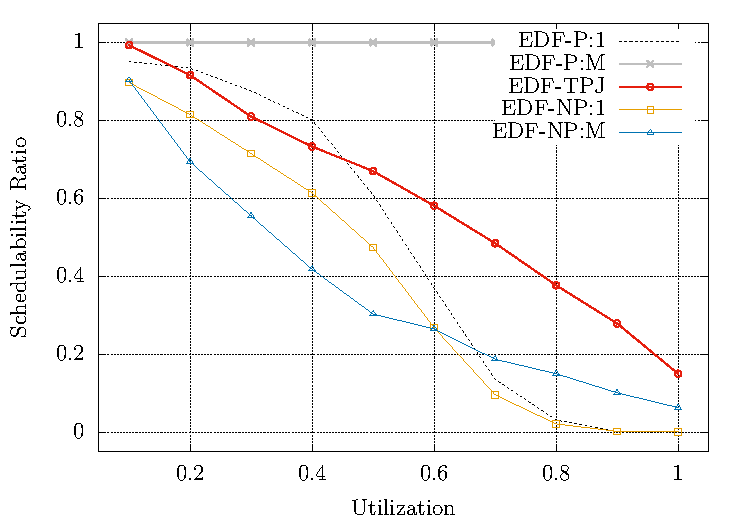
\includegraphics[width=\linewidth]{plot/cs-ratio/cs-ratio}
    \caption{\texttt{BUNDLEP} Case Study}
    \label{fig:cs-ratio}
  \end{subfigure}%
  \begin{subfigure}{\cwidth}
    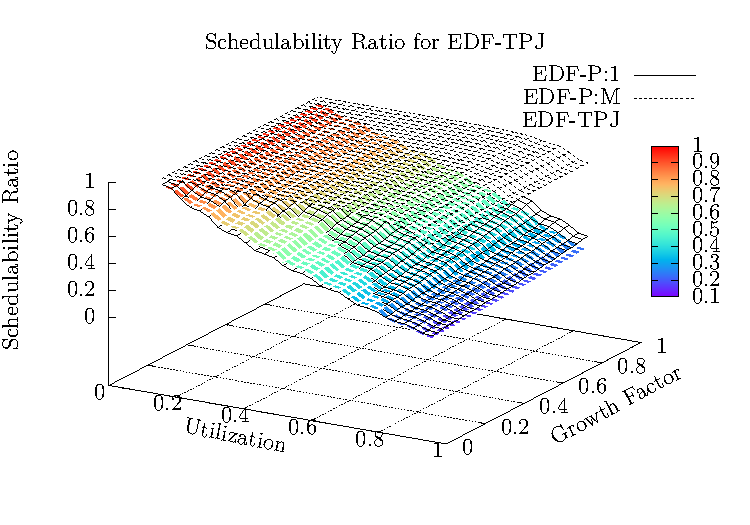
\includegraphics[width=\linewidth]{plot/avg-alg-sched/avg-ratio-TPJ-i}
    \caption{EDF-TPJ Summary}
    \label{fig:avg-ratio-TPJ-i}
  \end{subfigure}
  \caption{Case Study and EDF-TPJ Summary Results}
\end{figure}

Schedulability ratios from the \bundlep{} case study are given in
Figure~\ref{fig:cs-ratio}. For the target architecture and 18 benchmarks, EDF-TPJ consistently outperforms the other non-preemptive
algorithms. For preemptive EDF-P:1 (with zero cost preemptions), EDF-TPJ
has higher schedulability ratios for the majority of target
utilization values. EDF-TPJ's comparative performance increases
with the target utilization. This case study demonstrates the benefit
of \tpj{} to non-preemptive and (potentially) preemptive approaches.
 
Figures~\ref{fig:avg-ratio-TPJ-i}, \ref{fig:avg-ratio-NP-1}, and \ref{fig:avg-ratio-NP-m}, summarize the results for the synthetic
task sets varied by the utilization and growth factor. Within
each graph, the schedulability ratios provided by EDF-P:1 and EDF-P:M serve as
references. The difference between EDF-P:1 and the subject of the
graph illustrate the benefit of preemptive scheduling. Inclusion of
EDF-PM highlights the theoretical limit of concave growth to
schedulability.

\begin{figure}[hb]
  \centering
  \begin{subfigure}{\cwidth}
    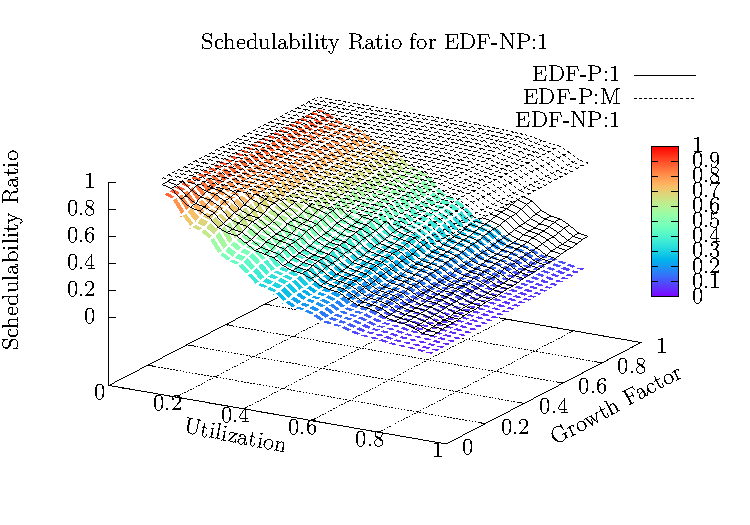
\includegraphics[width=\linewidth]{plot/avg-alg-sched/avg-ratio-NP-1}
    \caption{EDF-NP:1 Summary}
    \label{fig:avg-ratio-NP-1}
  \end{subfigure}%
  \begin{subfigure}{\cwidth}
    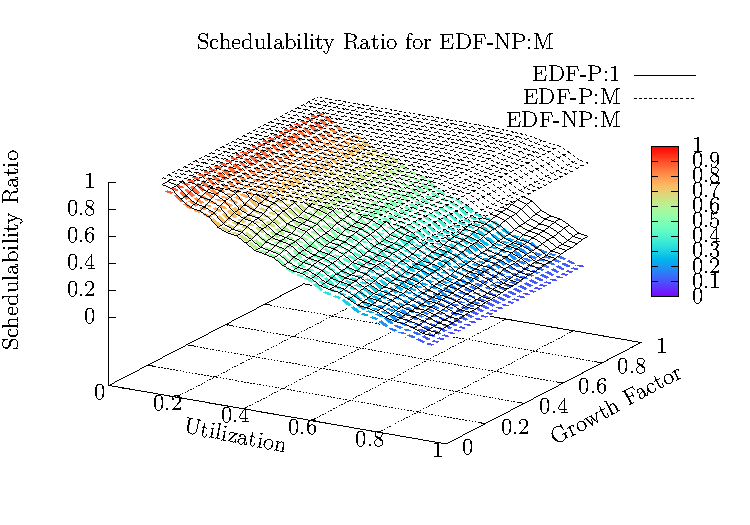
\includegraphics[width=\linewidth]{plot/avg-alg-sched/avg-ratio-NP-m}
    \caption{EDF-NP:M Summary}
  \label{fig:avg-ratio-NP-m}
  \end{subfigure}
  \caption{EDF-NP:1 and EDF-NP:M Summary}
\end{figure}

Including EDF-P:1 and EDF-P:M in each of the summary
graphs eases the comparison between EDF-NP:1, EDF-NP:M, and
EDF-TPJ. Comparing EDF-NP:1 (\ref{fig:avg-ratio-NP-1}) to EDF-NP:M
(\ref{fig:avg-ratio-NP-m}), illustrates the benefits of the model and
scheduling mechanism. EDF-NP:M has a consistently higher
schedulability ratio for all utilizations and growth factors. EDF-TPJ
(\ref{fig:avg-ratio-TPJ-i}) outperforms EDF-NP:M, with higher schedulability
ratios for all utilizations and growth factors due to the ability to
transform task sets. EDF-TPJ performs best among the non-preemptive
tests across all configurations. Additionally, EDF-TPJ is able to
schedule task sets deemed infeasible for EDF-P:1.

Table~\ref{table:by-m} summarizes the infeasible utilization
findings for the synthetic tasks. For moderate and larger values of
${M (\ge 25)}$, the number of infeasible by utilization task sets
dominate the specifications. For 25, 50, and 100 total threads, the
infeasible by utilization comprise 44, 59, and 74 percent of the task
sets respectively, with EDF-TPJ finding 25, 34, and 45 percent 
feasible. This illustrates the large potential of the proposed model,
in conjunction with concave growth WCET functions of
thread-level schedulers (e.g. \bundle{} and \bundlep{}).

\begin{figure}[ht]
  \centering
  \begin{tabular}{|r||c|c|c|c|c|c|c||l|}
\hline
${(M, m)}$ & ${(3, 2)}$ & ${(5, 2)}$ & ${(7, 3)}$ & ${(10, 4)}$ & ${(25, 8)}$ & ${(50, 16)}$ & ${(100, 32)}$ & Total \\
${|S|}$ & 81000 & 81000 & 81000 & 81000 & 81000 & 81000 & 81000 & 567000 \\
${|s|}$ & 3131 & 4973 & 11744 & 18689 & 36565 & 49147 & 59412 & 183661 \\
${|\stpj{}|}$ & 465 & 291 & 1437 & 3065 & 9426 & 16912 & 25832 & 57428 \\
\hline
\end{tabular}
\caption{${U > 1}$ Feasibility}
\label{table:by-m}
\end{figure}

There are two noteworthy trends within the schedulability results.
The simpler of the two is the relationship between utilization and
schedulability ratio for a fixed growth
factor. Figure~\ref{fig:M10F.5} illustrates the trend common among ${M
  \le 10}$ total threads. The trend for preemptive and non-preemptive
schedulability tests when utilization increases is for the
schedulability ratio to decrease. However, EDF-TPJ always outperforms 
the other non-preemptive tests. 

The second trend is slightly more complex. Figure~\ref{fig:M10U.5} was
selected for the smallest ${M}$ and ${U}$ values with visually
distinct plots per schedulability test. The growth factor and the
schedulability ratio are correlated. As the growth factor increases,
so does the schedulability ratio. This is due to the utilization being
held constant. When the growth factor is small, the WCET of the first
thread of each task is larger. Larger WCET values are harder to
schedule non-preemptively.  

\begin{figure}[ht]
  \centering
  \begin{subfigure}{\cwidth}
    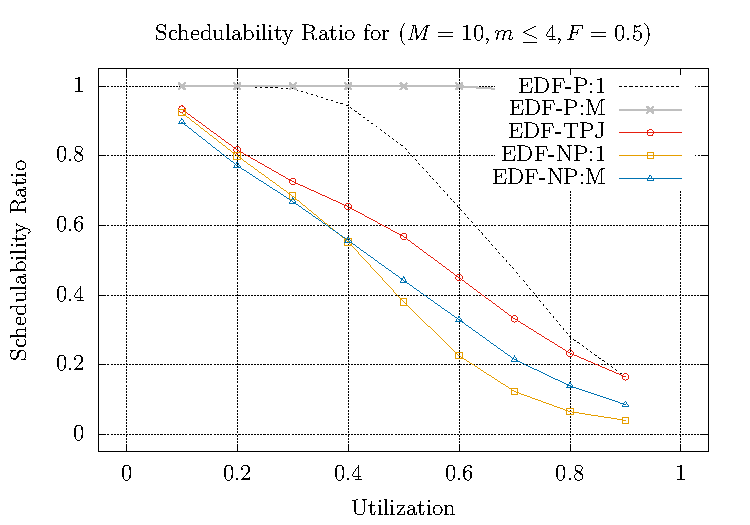
\includegraphics[width=\linewidth]{plot/2D-UFS/2D-M010m04F0_5xS}%
    \caption{${(M,m,U,\GFactor{}) = (10,4,*,0.5)}$}
    \label{fig:M10F.5}
  \end{subfigure}%
  \begin{subfigure}{\cwidth}
    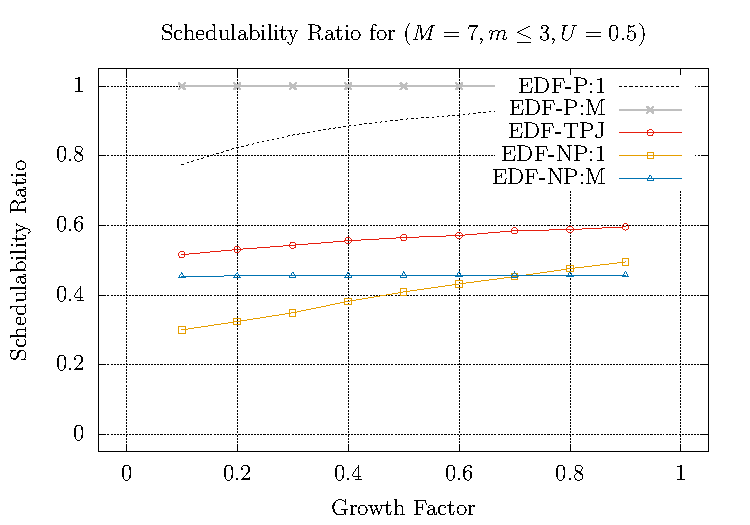
\includegraphics[width=\linewidth]{plot/2D-UFS/2D-M007m03U0_5xS.pdf}%
    \caption{${(M,m,U,\GFactor{}) = (7,3,0.5,*)}$}
    \label{fig:M10U.5}
  \end{subfigure}%
  \caption{${M \le 10}$ Performance}%
\end{figure}

\begin{figure}[ht]
  \centering
  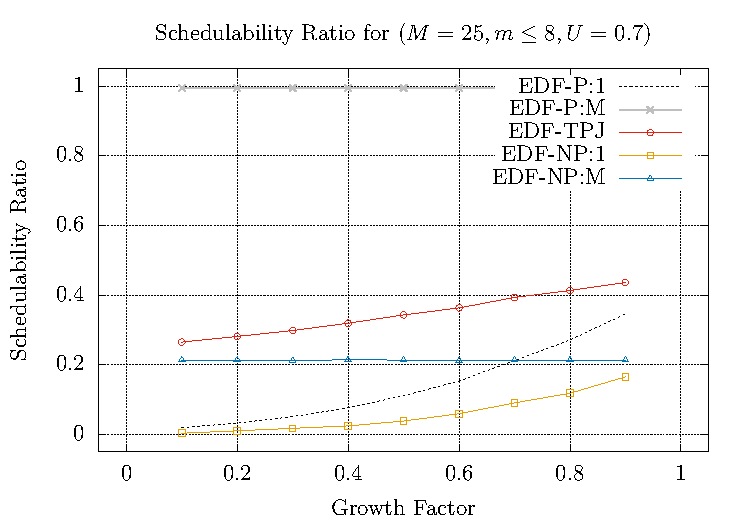
\includegraphics[width=\cwidth]{plot/2D-UFS/2D-M025m08U0_7xS}\quad
  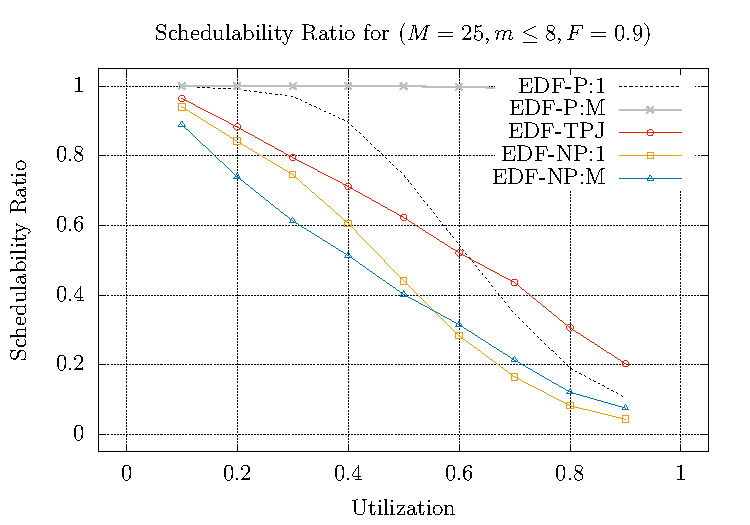
\includegraphics[width=\cwidth]{plot/2D-UFS/2D-M025m08F0_9xS}%
  \caption{${M > 10}$ EDF-TPJ Performance Above EDF-P:1}
  \label{fig:m25-tpj}
\end{figure}

\begin{figure}[ht]
  \centering
  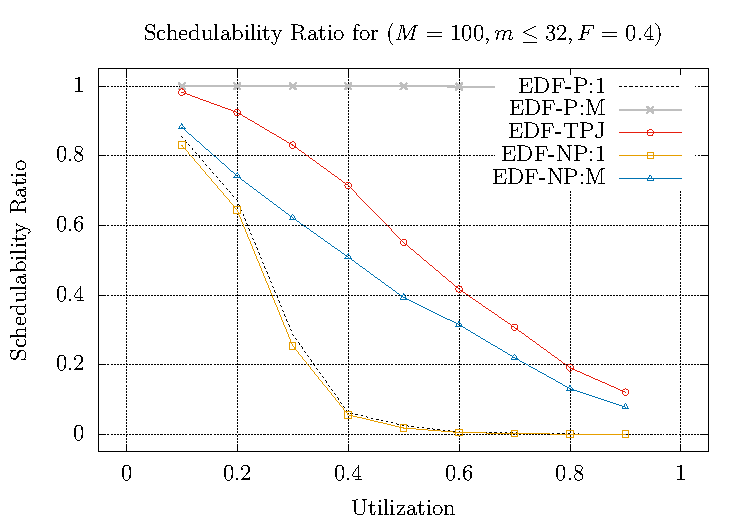
\includegraphics[width=\cwidth]{plot/2D-UFS/2D-M100m32F0_4xS}\quad
  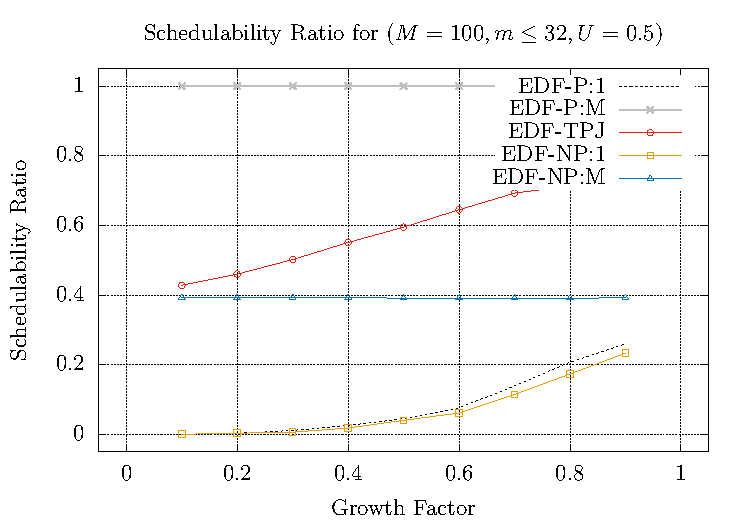
\includegraphics[width=\cwidth]{plot/2D-UFS/2D-M100m32U0_5xS}%
  \caption{${M = 100}$ EDF-TPJ Performance}
  \label{fig:m100-tpj}
\end{figure}

As ${M}$ increases beyond 10 total threads, the number of infeasible
by utilization task sets ${s}$ grows. This contributes to the
schedulability ratio of EDF-TPJ surpassing EDF-P:1 for
threshold utilization and growth factor values. For ${M = 25}$, the
threshold of utilization is between ${[0.6,0.7]}$ shown in
Figure~\ref{fig:m25-tpj}.

For ${M = 100}$ and ${\GFactor \le 0.4}$, EDF-TPJ outperforms
EDF-P:1. Figure~\ref{fig:m100-tpj} highlights the advantage of
EDF-TPJ compared to EDF-P:1 by virtue of concave growth. It also
highlights the benefit of dividing tasks, as the performance of
EDF-NP:M is always below EDF-TPJ.

The comparative performance of EDF-TPJ is at its lowest
for ${M < 10}$ threads and ${U > .4}$ utilization. In these ranges
EDF-TPJ maintains the highest schedulability ratio among the
non-preemptive methods, but the ratio is closer to EDF-NP:M or
EDF-NP:1 than EDF-P:1. This suggests, the decrease in EDF-TPJ's
performance is more likely due to the non-preemptive setting combined
with larger WCET values for individual threads.

%%%%%%%%%%%%%%%%%%%%%%%%%%%%%%%%%%%%%%%%%%%%%%%%%%%%%%%%%%%%%%%%%%%%%%
% Conclusion
%%%%%%%%%%%%%%%%%%%%%%%%%%%%%%%%%%%%%%%%%%%%%%%%%%%%%%%%%%%%%%%%%%%%%%
\section{Conclusion}\label{sec:conclusion}

Motivation for this work stemmed from \texttt{BUNDLE}-based
thread-level schedulers limitation of a single task and single
job. The primary goal was to create a multi-task scheduling technique
and schedulability test for those \texttt{BUNDLE}-based thread-level
schedulers which leverages without decreasing the inter-thread cache
benefit.

In addition to achieving the primary goal, the scheduling technique
and schedulability test developed for the multi-task
\texttt{BUNDLE}-based scheduler can be applied to any thread level
scheduler with strictly increasing discrete concave WCET
functions. This allows any compatible thread-level scheduling
technique to benefit from the \tpj{} approach developed in this
work. As a non-preemptive multi-threaded schedulability test \tpj{} is
optimal with respect to npm-feasibility, always producing a feasible
task set if one is schedulable by EDF-NP.

For future work, the primary focus is upon a fully or limited preemption
scheduling algorithm that permits the inter-thread cache benefit of
\texttt{BUNDLE}-based schedulers and other schedulers
characterized by concave growth to retain their thread-level
scheduling benefits.

\bibliography{main}
\end{document}
